% !TEX root = main.tex
\label{ch:campaigns}

Computational campaigns enact an execution plan to achieve a computational
objective for given requirements and constraints. A computational objective is a
set of values for a set of metrics that must be satisfied. Some of these metrics
are time to completion or throughput defined as number of workflows executed per
unit of time. Requirements, generally, describe the minimum amount and type of
resources needed to execute each workflow of the campaign, while constraints are
the conditions that bound the execution, such as resource availability, resource
capacity or costs.

The objective of a campaign can be translated to a computational objective
function that satisfies a lower or upper bound of a metric. Among the many
metrics that can be considered, the most common one is the total time taken to
execute all workflows of a campaign, also known as makespan. An execution plan
of a campaign is a mapping between workflows and resources on which to execute
those workflows. Calculating the makespan of a campaign for a given plan
means verifying if said execution plan satisfies the computational objective
function, within the given constraints.

% A computational campaign can utilize several resources concurrently. These
% resources can either be homogeneous or heterogeneous as they offer different
% type of computational resources. One aspect of this heterogeneity is the
% performance each resource has in terms of number of operations per second.
% High Performance Computing (HPC) resources, a campaign can utilize, offer the
% concurrent execution of workflows on different sets of the same type or
% different type of computational resources, thus homogeneous or heterogeneous
% respectively. Different types of computational resources can be offered by the
% same HPC resource or different HPC resources.

We focus on computational campaigns that can concurrently utilize several high
performance computing (HPC) infrastructures, i.e., supercomputers. Further, we
consider infrastructures with homogeneous and heterogeneous resources, depending
on the type of computational capabilities they offer, e.g., number of operations
per second. Each HPC infrastructure can offer a set of homogeneous or
heterogeneous resources and a set of HPC infrastructures can also be homogeneous
or heterogeneous.

% Uncertainty in the execution of a campaign can arise for several reasons,
% including resource dynamism and workflow runtime uncertainty. HPC resources
% are governed via policies that affect their performance, such as power
% regulating policies~\cite{inadomi2015analyzing} and filesystem and network
% multitenancy~\cite{brown2018interference}. As a consequence, their performance
% changes over time and is dynamic, which in turn creates uncertainty on the
% makespan of a campaign. Further, accurately estimating the runtime of each
% workflow in a campaign is challenging, as each workflow can have different
% inputs or datasets to analyze. Instead, users offer an estimation in the form
% of a range of possible values. Both resource dynamism and workflow runtime
% uncertainty have the potential to increase the makespan of an execution plan.

Uncertainty about the makespan of a campaign arises from two main reasons:
resource dynamism and workflow runtime estimation. HPC resources are governed by
policies that affect their performance, such as power regulating
policies~\cite{inadomi2015analyzing} and filesystem and network
multitenancy~\cite{brown2018interference}. As a consequence, resource
performance changes over time (i.e, is dynamic) which, in turn, creates
uncertainty about the makespan of a campaign. Further, accurately estimating the
runtime of each workflow of a campaign is challenging at best, impossible at
worse. Users offer an estimation of each workflow runtime in the form of a range
of possible values which, in turn, also creates uncertainty about the makespan
of a campaign.

% Deriving an execution plan for a campaign before its execution on dynamic and
% heterogeneous resources, while workflows runtime are uncertain, is challenging.
There is a plethora of algorithms which derive an execution plan by calculating
the makespan of a workflow offline~\cite{lu2019review}, i.e., before the
workflow's execution. Planning for a campaign with $N_W$ workflows is equivalent
to planning for a workflow with $N_t$ tasks. Offline algorithms usually take
information about resource performance and task/workflow runtime as input, and
use that information to produce a plan. As a result, the plan produced can be
significantly affected by the uncertainty described above.
% when resource performance changes over time and/or when the workflow runtime
% estimation is uncertain.

% Having an understanding of how plans from different algorithms perform in such
% an execution environment is important.
To the best of our knowledge, there is not a methodology that allows to compare
planning algorithms on dynamic heterogeneous resources and in presence of
workflows runtime estimation uncertainty. We select three algorithms, each
representing a family of algorithms, and compare their performance in respect to
the makespan of the plans they produce as well as how sensitive they are on
resource dynamism and workflows runtime uncertainty. Based on the comparison, we
make a case about which algorithm to select given a computational campaign, the
execution environment, constraints and objective.

The chapter is organized as follows:~\S\ref{sec:camp_rw} discusses related
work. ~\S\ref{sec:makespan_calc} discusses the
calculation of the makespan of a campaign given the set of assumptions of this
work. Section~\S\ref{sec:algo} discusses three makespan calculation algorithms
and~\S\ref{sec:algo_perf_comp} compares their performance. Finally,
section~\S\ref{sec:cf_algo_sel} presents our conclusions and a conceptual
framework that will allow users to best select a planning algorithm. The chapter
offers the two main contributions:
\begin{inparaenum}[(i)]
    \item an experimental methodology to compare the performance of planning
    algorithms that is independent of the considered use case and computing
    framework; and
    \item a conceptual framework for selecting planning algorithms based on the
    algorithmic, campaign and resources characteristics.
\end{inparaenum}


\section{Related Work}
\label{sec:camp_rw}

Several methods compare and evaluate algorithms that calculate and optimize the
makespan of a workflow~\cite{lu2019review}, including queuing
networks~\cite{yao2019throughput,bao2019performance}, domain specific
languages~\cite{carothers2017durango,maheshwari2016workflow}, and machine
learning~\cite{witt2019predictive,pumma2017runtime}. Queuing networks are of
limited use because they require from the user to provide a queuing network
equivalent to the campaign. In the case the campaign contains only independent
workflows, a single queuing system with multiple servers would be sufficient,
but a campaign with complex dependencies among workflows may require expertise
outside the user's domain to define the equivalent queuing network. Furthermore,
using queuing methods to derive the makespan of a campaign requires to search
for possible mappings and keep the one that optimizes the makespan. Domain
specific languages approaches either require description of the resource usage
of workflows~\cite{carothers2017durango}, or to execute part of the campaign to
obtain an execution ``skeleton''~\cite{maheshwari2016workflow}.
When executing a campaign, workflows may require days to execute to obtain
execution time information, and users rarely know the resource usage of their
workflows to provide accurate enough information.

Some work has been done to evaluate different planning algorithms.
Ref.~\cite{wieczorek2005scheduling} offers a survey of different algorithms for
planning the execution of workflows on Grid resources.
Ref.~\cite{canon2008comparative} experimentally compares a set of
makespan-centric, heuristic-based planning algorithms. Algorithms are ranked
based on how robust they are when task runtimes are uncertain. This approach is
very close to our approach but we do not limit our evaluation to a specific type
of algorithm and we also measure how planning algorithms perform in presence of
resource dynamism and workflow runtime estimation uncertainty.

% ------------------------------------------------------------------------------
\section{Calculating the Makespan of a Campaign}
\label{sec:makespan_calc}

The way workflows of a given campaign are mapped to resources can affect the
makespan calculation. Figure~\ref{fig:example_makespan} shows an example of a
campaign with workflows of different size and execution times, and the makespans
that two different mappings produce. The makespan of the campaign on the left
sub~-figure is $20$, while that on the right it is $16$. In addition,
Figure~\ref{fig:example_makespan} also shows the relevance of the size of the
workflows, i.e., the number of resources they require, and that resources may be
underutilized.

\begin{figure*}[ht!]
    \centering
    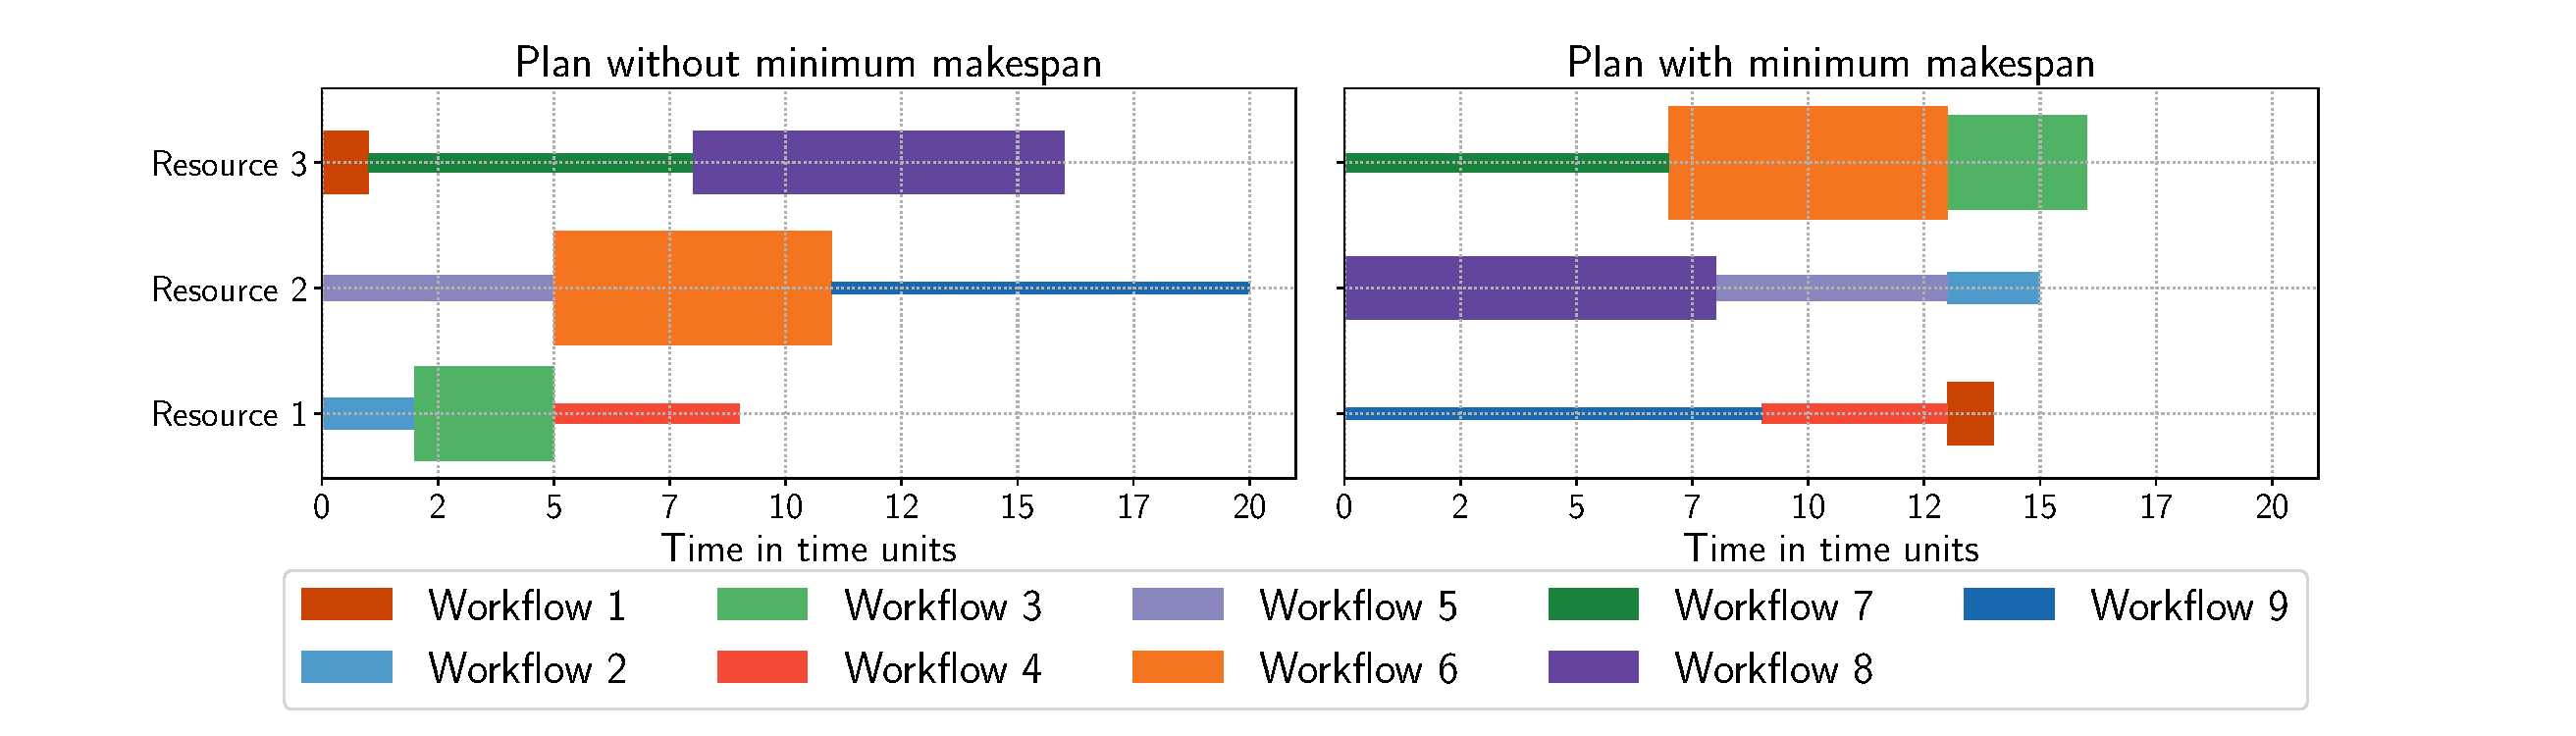
\includegraphics[width=.99\textwidth]{figures/campaign/plan_comp.pdf}
    \caption{Comparison of different campaign execution plans. Makespan and
    resource utilization is different, based on workflow mapping on
    resources.}\label{fig:example_makespan}
\end{figure*}

We make a set of assumptions when defining a model for the calculation of a
campaign makespan:
\begin{inparaenum}[(1)]
    \item a workflow is an atomic unit;
    \item a workflow resource request is always sufficient to execute the
    workflow;
    \item a resource is an aggregate of computing capabilities;
    \item every workflow of a given campaign can be executed on the given
    resources;
    \item random resource selection is based on a uniform distribution;
    \item only one workflow can be executed on a resource at any point in time;
    and
    \item workflows can be homogeneous or heterogeneous in time---the amount of
    time they are executing---and space---the amount of resources they require.
\end{inparaenum}

We denote a computational campaign as $C = [w_{i}: 1 \leq i \leq N_{C}]$,
where $w_{i}$ is a workflow and $N_{C}$ is the total number of workflows,
$R = [ r_{j}: 1 \leq j \leq N_{R}]$ is a set of available resources, where
$r_{j}$ is a resource and $N_{R}$ is the total number of available resources
before the execution of the campaign. $M(C,R)$ is a mapping function
which produces a map $ [(w_i, r_j): 1 \leq i \leq N_{C}, r_j \in R] $ of
workflows onto resources. In addition, we denote the execution time of a
workflow as $Tx_{w_{i}}$, the makespan of campaign $C$ as $TTX_{C}$, and the
makespan of campaign $C$ for a given mapping function $ M $ as $TTX_{C}(M)$.

With a single resource, i.e., $N_{R} = 1$, the workflows of a campaign are
executed sequentially, regardless of the execution order or whether the
workflows are homogeneous or heterogeneous. As a result the makespan of the
campaign is:
\begin{equation}
   TTX_{C} = \sum_{i=1}^{N_{C}}Tx_{w_{i}}
\end{equation}

With multiple resources, i.e., $1 < N_{R} < N_{C}$, the workflows of a campaign
can be executed concurrently. With homogeneous resources, this is semantically
equivalent to executing the campaign on a single resource large enough to allow
concurrent workflow execution, where each workflow executes on a resource
partition. Because of assumptions~\#4 and~\#7, the execution of spatially
homogeneous or heterogeneous workflows has the same makespan. A random mapping
of workflows onto resource has a makespan:
\begin{equation}
   TTX_{C}(Random) \geq \frac{1}{N_{R}}\sum_{i=1}^{N_{C}} Tx_{w_{i}}
\end{equation}

Given multiple homogeneous resources, when executing workflows that are
heterogeneous in time and that can be spatially homogeneous or heterogeneous,
the makespan of the campaign for a given mapping function $M$ is:
\begin{equation}
TTX_{C}(M) = \max_{r_{j}\in R}\Big\{\sum_{w_{i}\in M(C,r_{j})}Tx_{w_{i}}\Big\}
\label{eq:makespan}
\end{equation}
Relaxing the assumption that resources are heterogeneous, in the performance
they offer, affects the result of the mapping function $M$. As a result,
Eq.~\ref{eq:makespan} holds in calculating the makespan of the campaign.

%Computational campaigns execute to achieve an objective.
%We consider as objective the total time of completion of the campaign.
%As a result, the objective function of a plan is translating in minimizing the value of eq~\ref{eq:makespan}.
%The objective function is:
%\begin{equation}
%    \min\Big\{\max_{r_{j}\in R}\Big\{\sum_{w_{i}\in M(C,r_{j})}Tx_{w_{i}}\Big\}\Big\}
%\end{equation}
%In the next section, we discuss a set of algorithms that try to satisfy this objective function.

% -------------------------------------------------------------------
\section{Planning Algorithms}
\label{sec:algo}

We investigate three algorithms: (i) the Heterogeneous Earlier Finish Time
algorithm (HEFT)~\cite{topcuoglu2002performance}; (ii) a genetic
algorithm~\cite{page2005algorithm}; and (iii) a simple heuristic algorithm. These algorithms produce an execution plan before the actual execution of
the campaign, and require workflow runtime and resource performance as input.
Table~\ref{tab:sched_algo} shows a summary of the algorithms characteristics.

\begin{table}[t]
    \centering
    \scriptsize
    \begin{tabular}{@{}lcccc@{}}
        \toprule
                                   &
        \textbf{HEFT}              &
        \textbf{Genetic Algorithm} &
        \textbf{L2FF}              &
        \textbf{Random}            \\
        \midrule
        Decision Policy       &
        Deterministic         &
        Convergence Criteria  &
        Deterministic         &
        Deterministic         \\
        %
        Initial State         &
        Blank                 &
        Semi-random           &
        Blank                 &
        Blank                 \\
        \midrule
        \multicolumn{5}{@{}l}{\textbf{Initial Information}} \\
        \midrule
        Workflow Operations   &
        Yes                   &
        Yes                   &
        Yes                   &
        No                    \\
        %
        Resource Performance  &
        Yes                   &
        Yes                   &
        Yes                   &
        No                    \\
        \midrule
        Produced Knowledge    &
        Resource availability &
        Resource availability &
        None                  &
        None                  \\
        \bottomrule
    \end{tabular}
    \caption{Basic characteristics of selected planning algorithms.}
    \label{tab:sched_algo}
\end{table}

% -------------------------------------------------------------------
\subsection{Heterogeneous Earlier Finish Time (HEFT) algorithm}
\label{algo:heft}

List scheduling algorithms represent a family of heuristic-based algorithms to
schedule workflows~\cite{dong2006scheduling,list_sched_wiki}. These algorithms
assign priorities to tasks based on a heuristic and then order tasks based on
their priority. To place tasks on resources, they traverse the ordered list of
tasks and assign a task to a resource that can execute it. HEFT is a list
scheduling algorithm~\cite{dong2006scheduling} and calculates the makespan of a
workflow on heterogeneous resources to produce its plan.

Pegasus~\cite{deelman2015pegasus} and ASKALON~\cite{fahringer2005askalon}
utilize HEFT to derive workflow execution plans amongst other algoirthms, such
as Round Robin, a genetic algorithm and a myopic algorithm. HEFT
has been shown to provide better performance in terms of makespan minimization
compared to other mapping
algorithms~\cite{topcuoglu2002performance,canon2008comparative}, e.g., genetic
algorithms~\cite{fahringer2005askalon}. Furthermore, there is initial
research to extend HEFT to dynamic resources~\cite{dong2007pfas}, and to
resources that provide CPU and GPUs~\cite{shetti2013optimization}.

HEFT makes two assumptions when used on workflows:
\begin{inparaenum}[(1)]
    \item any task in a workflow can be executed on all available resources; and
    \item all resources are initially available.
\end{inparaenum}
HEFT's complexity is proportional to the number of dependencies among tasks
and the number of resources offered. As we are interested in executing
computational campaigns, our HEFT extension provides an execution plan based
on workflows as atomic units instead of tasks. Algorithm~\ref{alg:heft} shows
HEFT for placing independent workflows on resources.

\begin{algorithm}[t]
    \caption{Heterogeneous Earliest Finish Time (HEFT) algorithm}
    \label{alg:heft}
    \scriptsize
    \begin{algorithmic}[1]
        \Procedure{HEFT}{$W$,$R$}\Comment{$W$ and $R$ are a set of workflows and resources respectively}
        \State \texttt{Calculate the computation cost $w_{tx}^{ij}$ of each workflow for all resources}
        \State \texttt{Assign $rank_i = \overline{w_{i}} = \nicefrac{\sum_{j=1}^{|R|}w_{tx}^{ij}}{|R|}$}
        \State \texttt{Sort workflows in decreasing order of $rank_i$}
        \While{unscheduled workflows}
        \State \texttt{Select the first workflow $\tilde{w}$ from the sorted list}
        \For{$\forall r_{j}$ in $R$}
        \State\texttt{Compute earliest finish time for $\tilde{w}$ on $r_{j}$, $eft_{\tilde{w},r_j}$ }
        \EndFor
        \State \texttt{Assign  $\tilde{w}$ on $r_k$ with $\min{(eft_{\tilde{w},r_j})}$}
        \EndWhile
        \EndProcedure
    \end{algorithmic}
\end{algorithm}

HEFT has three main algorithmic characteristics:
\begin{inparaenum}[(1)]
    \item creates a priority list of workflows;
    \item produces an expectation of when resources are available; and
    \item uses a deterministic heuristic.
\end{inparaenum}
Initially, HEFT calculates the average execution time of a workflow on all
resources and creates a priority list with the longest workflow first. In
addition, HEFT initializes a vector with information about where each workflow
is when a resource is available. Then, HEFT calculates when a workflow will
finish at each resource and places that workflow on the resource that will finish
it earlier. HEFT ends when all workflows are placed on a resource.


% -------------------------------------------------------------------
\subsection{Genetic Algorithm}
\label{algo:gen}

Genetic algorithms are another family of algorithms that can be  used to
calculate the makespan of workflows~\cite{dong2006scheduling}. Genetic
algorithms start from an initial set of possible solutions, and iterate and
improve them across multiple iteration. In our case, genetic algorithms follow
the following procedure:
\begin{inparaenum}[(i)]
    \item create an initial population, where the population is a set of
    possible plans;
    \item evaluate the population members based on a fitness function, which
    calculates the makespan of the workflow;
    \item reproduce by selecting population members, either randomly or based
    on their fitness value, and generate a new set of possible plans; and
    \item mutate, where randomly selected tasks from a random population
    member are reassigned to resources.
\end{inparaenum}

The selected genetic algorithm~\cite{page2005algorithm} was developed to support
the placement of independent tasks on heterogeneous resources. It assumes that
all tasks that can be executed on all available resources, are independent and
indivisible. These assumptions are consistent with the assumptions we made for
the workflows in a campaign and we therefore extend this algorithm to support
scientific campaigns. The pseudocode of the selected genetic algorithm is shown
in Algorithm~\ref{alg:gen_algo}.

\begin{algorithm}[t]
    \caption{Genetic Algorithm}
    \label{alg:gen_algo}
    \scriptsize
    \begin{algorithmic}[1]
        \Procedure{GA}{$W$, $R$}\Comment{$W$ and $R$ are a set of workflows and resources respectively}
        \State \texttt{Initialize population}
        \While{Conergence Criteria not met and \#Gen $<$ Total\_Generations}
        \State{Selection}
        \State{Reproduce}
        \State{Randomly mutate}
        \EndWhile
        \EndProcedure
    \end{algorithmic}
\end{algorithm}

The members of the initial population are constructed either randomly or
semi-randomly. Specifically for each individual member of the population,
a percentage of the workflows are randomly assigned
to resources, where the assignment is drawn from a uniform distribution and the
rest of the workflows are assigned based on an earlier finish time (EFT)
heuristic, similar to the one used by HEFT. The size of the population, i.e.,
potential plans, is set to 20 members. Ref.~\cite{zomaya2001observations} shown
that a population size of 20 members reduces the computational load of the
genetic algorithm without significantly impacting the final result.

Genetic algorithms use a fitness function to calculate the fitness of a
population member to its environment, returning a value between 0 and 1. In our
case, the fitness function calculates the distance of the makespan of a plan
from the ideal makespan. This distance is defined as:
\begin{equation}
E = \sqrt{(\sum_{j=1}^{N_{C}}Tx_{w_{j},r_{j}} - IM)^2}
\label{eq:fitness}
\end{equation}
where $N_{C}$ is the number of workflows and $IM$ is the ideal makespan. The
ideal makespan is equal to:
\begin{equation}
IM = \frac{\sum_{i=1}^{N_{C}}Tx_{w_{i}}}{\sum_{j=1}^{N_{R}}r_{j}}
\label{eq:ideal_fitness}
\end{equation}
The fitness of a plan is the equal to $F = 1/E$ when $E > 0$, otherwise to $F =
1$.

The algorithm selects members to reproduce based on their fitness values. The
fitness value of each member defines the probability of that member to be
selected. When the selection is complete, the algorithm uses cyclic
rotation~\cite{oliver1987study} to generate new population members and replaces
those with the lowest fitness.
% After, a population member is randomly selected and two random workflows swap
% \mtnote{workflows appear out of the blue. }, completing the mutation step.
The algorithm stops evolving either when a member has fitness equal to 1 or
after a specified number of iterations.

Our genetic algorithm has the following characteristics:
\begin{inparaenum}[(1)]
    \item creates partial plans randomly;
    \item produces an expectation of when resources are available;
    \item evolves plans randomly; and
    \item terminates based on a convergence criteria
\end{inparaenum}

\subsubsection*{Genetic Algorithm Convergence Rate for Different Configurations}

During the initialization phase of the genetic algorithm, we can select the
percentage of workflows that will be assigned through the EFT heuristic. This is
true for every member, i.e., plan, of the genetic algorithm population. We
expect that the percentage of non-random placement affects the final plan
selected by the genetic algorithm. We executed an experiment to measure the
convergence rate of the genetic algorithm when planning a campaign with
homogeneous workflows on homogeneous resources. In this case, distributing
equally the workflows on resources produces a plan with the ideal makespan as
defined in Eq.~\ref{eq:ideal_fitness}.

We use three configurations of our genetic algorithm: GA, GA-25 and GA-50. These
configurations differ by the percentage of workflows non-randomly assigned to
resources during the initialization of the population. GA makes no random
workflow assignment to resources while GA-25 assigns 25\% of the workflows
non-randomly and 75\% randomly, and GA-50 assigns 50\% of the
workflows non-randomly and 50\% randomly.

%non-randomly assigned for each individual plan of the population \mtnote{That
%sentence makes no sense: to what 'of the population' refers to? Percentage?}. We
%use 0~\% (GA), 25~\% (GA-25) and 50~\% (GA-50) \mtnote{This makes no sense too:
%percentage of what? And what is a GA? You are missing two sentences: We use four
%implementations of our genetic algorithm: GA, GA-..., ..., .... Those
%implementations differ by the percentange of ... etc.}.

Figure~\ref{fig:ga_conv1} shows the convergence rate of the genetic algorithm as
the number of workflows changes while the number of resources is constant. When
the population is initialized randomly, GA does not always equally distribute
workflows to resources, as the convergence rate is always less than 1. As a
result, GA does not always produce a plan with the ideal makespan. On the
contrary, GA-25 and GA-50 have a convergence rate of 1. The convergence rate of
GA-25 shows a drop for 8 and 16 workflows, but remains above 0.97 which allows
us to conclude that GA-25 does produce plans with the ideal makespan.

%Apart from a small drop, GA-25 shows 8, 16 and 32 workflows \mtnote{what does
%'showing 8, 16 and 32 workflows' mean?}. The drop is less than 0.03
%\mtnote{what is the unit of measure? 0.03 potatoes? ;)} which is not
%significant to conclude that GA-25 does not produce plans with the ideal
%makespan.

\begin{figure*}[ht!]
    \centering
    \begin{subfigure}[b]{0.75\textwidth}
        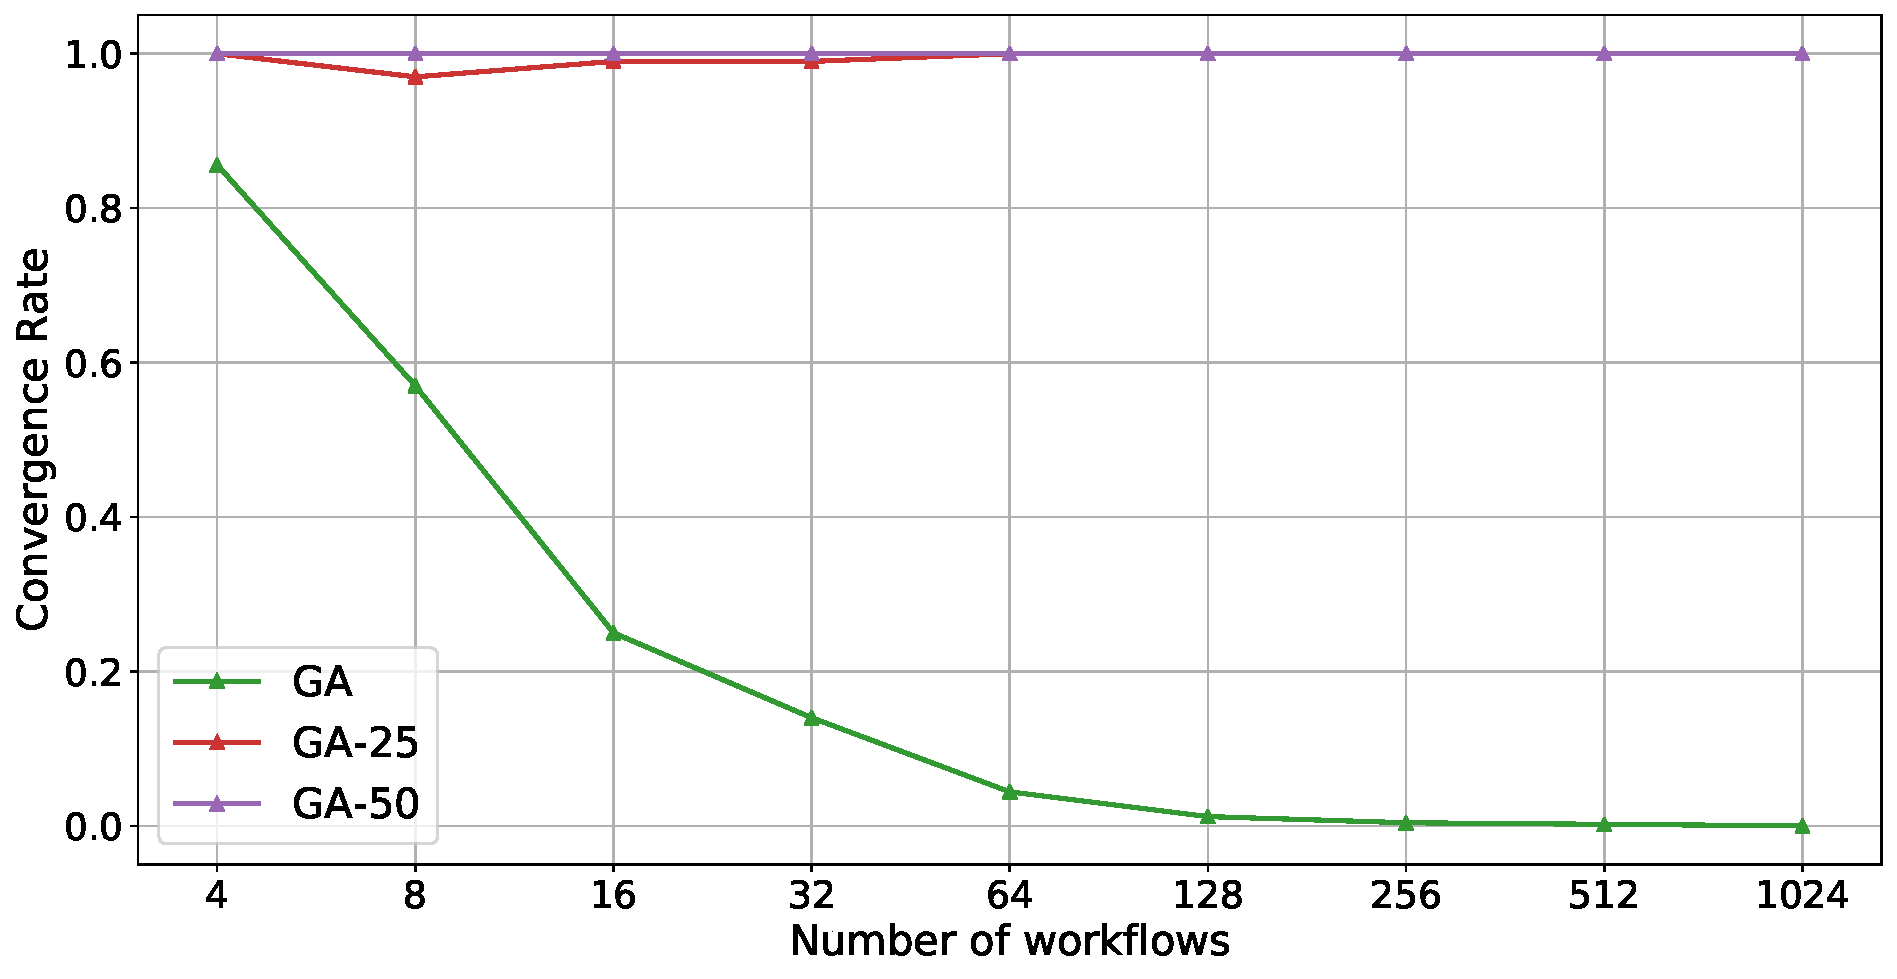
\includegraphics[width=.95\textwidth]{figures/campaign/StHomoCampaigns_4StHomoResourcesGAconv.pdf}
        \caption{}
        \label{fig:ga_conv1}
    \end{subfigure}\\
    ~
    \begin{subfigure}[b]{0.75\textwidth}
        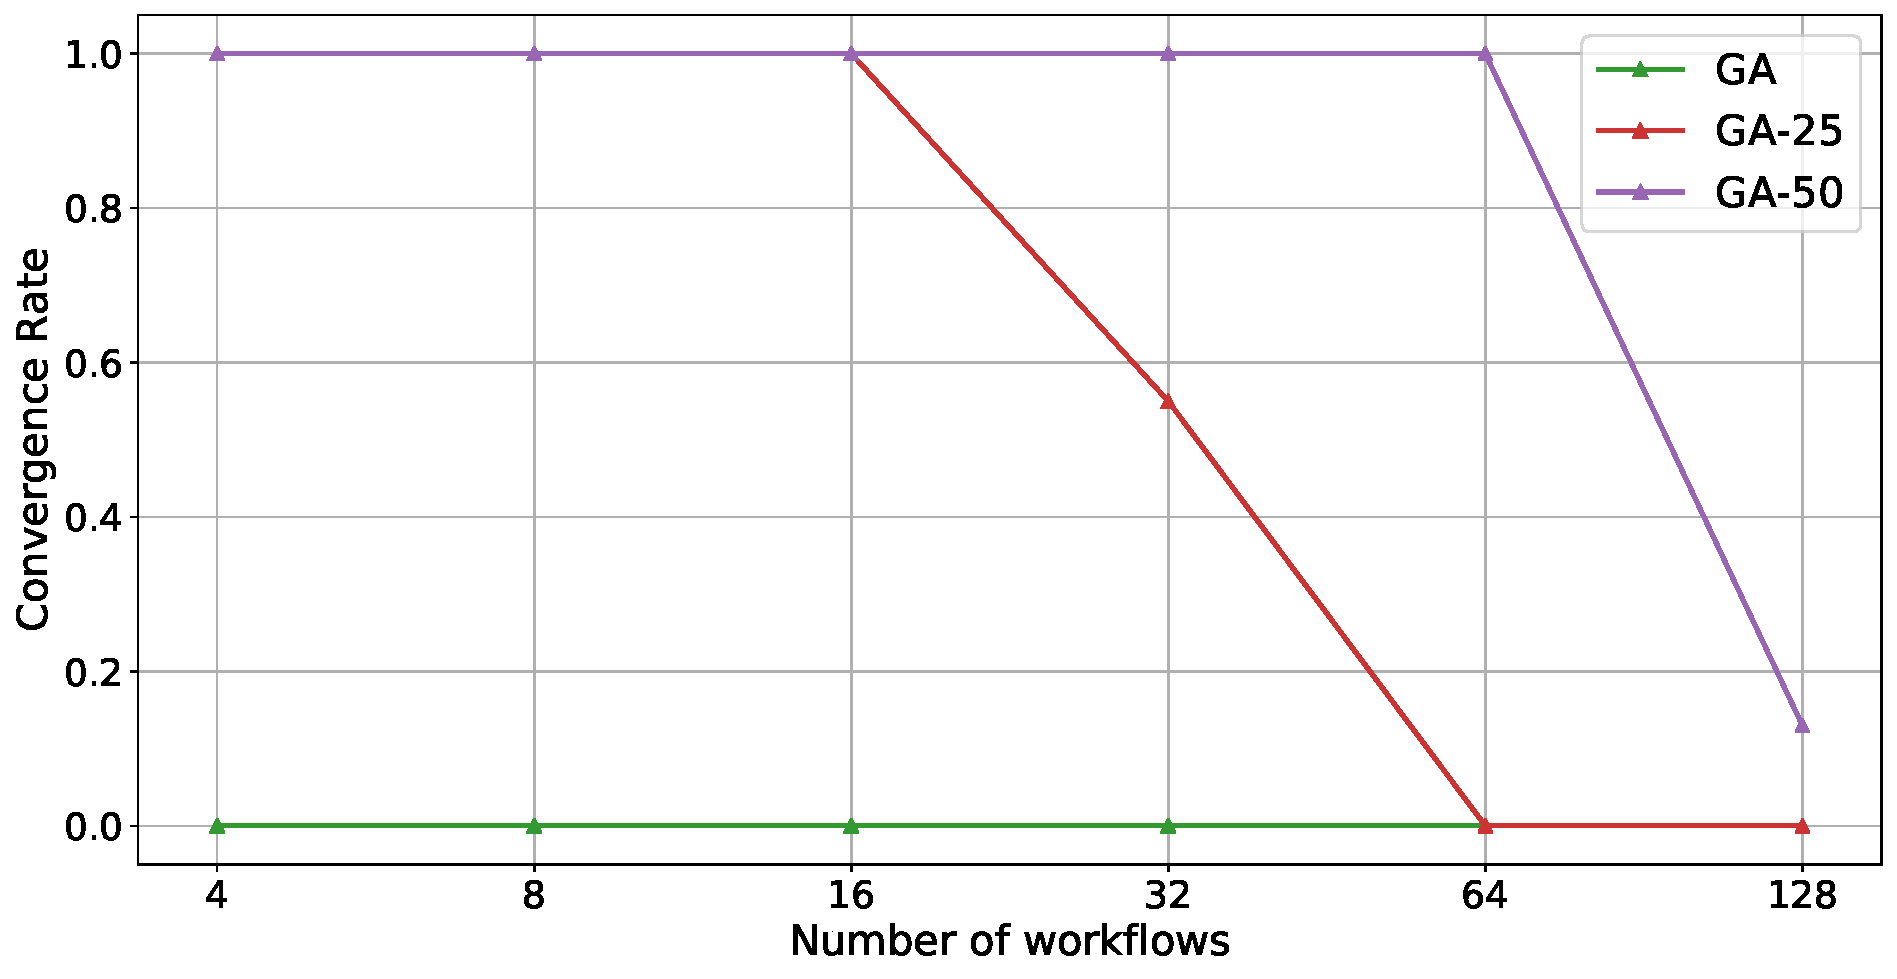
\includegraphics[width=.95\textwidth]{figures/campaign/HomogeResources_StHomogeCampaignsGAconv.pdf}
        \caption{}
        \label{fig:ga_conv2}
    \end{subfigure}
    \caption{Convergence rate of Genetic algorithm for homogeneous campaigns on
    static homogeneous resources based on random initialization
    percentage. \ref{fig:ga_conv1}) Different campaign sizes on 4
    resources;~\ref{fig:ga_conv2}) Campaign with 1024 workflows and different
    number of resources.}
    \label{fig:conv_rate}
\end{figure*}

Figure~\ref{fig:ga_conv2} shows the convergence rate of the genetic algorithm as
the number of resources changes while the number of workflows is constant. When
the population is randomly initialized, the genetic algorithm does not produce a
plan that has the ideal makespan. The convergence rate of GA-25 is 1 up to 16
resources and drops to 0 for more than 32 resources. GA-50 convergence rate is 1
up to 64 resources and drops to less than 0.2 for 128 resources and equal to 0
for 256 resources. The drop is due to the random initial placement of workflows
on resources. As the number of resources increase, the probability for GA to
place less than $N_{C} \ N_{R}$ workflows on a resource decreases.

Based the convergence rate, we expect that GA will not provide on average a plan
with the ideal makespan whether the campaign size or the number of resources
changes. GA-25 will provide plans with the ideal makespan when the number of
resources is less than 16, regardless the number of workflows. Finally, GA-50
will provide plans with ideal makespan up to 64 resources. Note that less than
ideal plans may still be desirable compared to those produced by other
algorithms.

% -------------------------------------------------------------------
\subsection{Longest to Fastest First Available Resource Algorithm}
\label{algo:l2ff}

The last algorithm we considered is an heuristics algorithm that places the
longest workflow on the fastest first available resource
(L2FF)~\cite{balasubramanian2019programming}. This algorithm sorts the workflows
based on the number of operations or workflow runtime estimation, and sorts
resources based on their performance. Then it places each workflow on the first
fastest available resource, starting from the longest workflow. A resource is
considered available when it has less or equal number of workflows than any
other resource. When workflows and resources are sorted, the placement is
equivalent to a modulo operation between the position of the workflow in the
sorted list and the number of resources. Algorithm~\ref{alg:l2ff} show the
pseudocode for this algorithm.

\begin{algorithm}[ht]
    \caption{Longest to Fastest First (L2FF)}
    \label{alg:l2ff}
    \begin{algorithmic}[1]
        \Procedure{l2ff}{$W$, $R$}\Comment{$W$ and $R$ are a set of workflows and resources respectively.}
        \State \texttt{$W_{sorted}=sort(W)$}
        \State \texttt{$R_{sorted}=sort(R)$}
        \For{$w$ in $W_{sorted}$}
        \State{Assign $w$ to $r_{k}$ where $k=w_{idx} \mod N_{R}$}
        \EndFor
        \EndProcedure
    \end{algorithmic}
\end{algorithm}

L2FF has the following algorithmic characteristics:
\begin{inparaenum}[(1)]
    \item creates a priority list of workflows; and
    \item uses a deterministic heuristic.
\end{inparaenum}
Contrary to HEFT and GA, L2FF does not produce an expectation of when a resource
is available because it does not calculate when each resource will be available
based on the duration on the workflow that is executed on that resource. This
reduces considerably the burden on the user and has the potential to simplify
the design and implementation of the campaign manager. Depending on its
performance, it may therefore be the preferable option to adopt.

% -------------------------------------------------------------------
\section{Performance Evaluation of Planning Algorithms}
\label{sec:algo_perf_comp}

We execute three experiments to evaluate and analyze the performance of the
selected algorithms. We use random plans as the baseline of our experiments.
The Random planner randomly selects a resource and places a workflow to that
resource. In addition, it requires no information about workflow runtime and
resource performance.

The first experiment measures the makespan of a plan that uses HEFT, GA, L2FF
and Random for different campaign and resource sizes. The second experiment
measures the sensitivity of the makespan to resource dynamism, i.e., resource
performance changes over time. We define sensitivity as the difference between
the makespan measured via executing a campaign and the expected makespan given
by the execution plan. Last, we measure the sensitivity of the makespan to
workflow runtime uncertainty. This set of experiments provides a methodology to
compare planning algorithms and decide which algorithm is more suitable, based
on the computational requirements of a campaign, e.g., workflow size, resource
performance and workflow runtime estimate.

We make a set of assumptions about resource performance and workflow runtime.
These assumption are based on the use cases we support and the capabilities of
the high performance computing resources we have access to. Resources can be
homogeneous or heterogeneous and static or dynamic. Resources are homogeneous
when they have the same performance in terms of operations per second,
heterogeneous otherwise. Resources are static when their performance does not
change over runtime and dynamic when it does. When resources are homogeneous, we
assume that their performance is equal to 1 petaFLOP. We use four existing HPC
resources as the basis for generating heterogeneous resources. These resources
are PSC Bridges, SDSC Comet, TACC Stampede2 and TACC Frontera with 
performance of 1.3~\cite{bridges_perf}, 2.7~\cite{comet_perf}, 10.6~\cite{top500}
and 23.5~\cite{top500} petaFLOPS respectively.

Workflow execution runtime is based on the use case described
in~\S\ref{ch:designs}. We measured the runtime of the use case by executing the
actual workflows on PSC Bridges. We adjusted the mean execution time and its
variance to an resource with performance of 1 petaFLOP and obtained a mean
runtime of 75000 seconds and a variance of 6000 seconds. For the purpose of our
experiments, we assume that workflow runtimes of a campaign are drawn by a
normal distribution with a mean and variance based on this use case. 

\subsection{Experiment 1: Measuring Makespan on Static Resources}

In our first experiment, we assume static resources and we use HEFT, GA, L2FF
and Random to measure the makespan for different campaign and resource sizes. We
use two configurations: in the first, we increase the size of the campaign from
4 to 2048 workflows, keeping the number of resources constant to 4; in the
second configuration, we increase the number of resources from 4 to 256
resources and we fix the campaign size to 1024 workflows.

%\subsubsection*{Homogeneous Campaign -- Homogeneous Resources}

We measure the makespan of executing a homogeneous campaign with workflows that
all have a runtime of 75000 seconds, on homogeneous resources with performance
of 1 petaFLOP. In this case, an algorithm produces the minimum makespan when it
equally distributes workflows to resources. Figure~\ref{fig:st_homog_analysis}
shows the makespan for plans which use HEFT, GA (50\% of the workflows are placed
randomly), L2FF and Random (RA).
Figure~\ref{fig:StHomoCampaigns_4StHomoResources} varies the campaign size from
4 to 2048 workflows with 4 resources, and
figure~\ref{fig:StHomoResources_StHomoCampaigns} varies the number of resources
from 4 to 256 resources with a campaign size equals to 1024 workflows.

\begin{figure}[ht!]
    \centering
    \begin{subfigure}[b]{0.75\textwidth}
        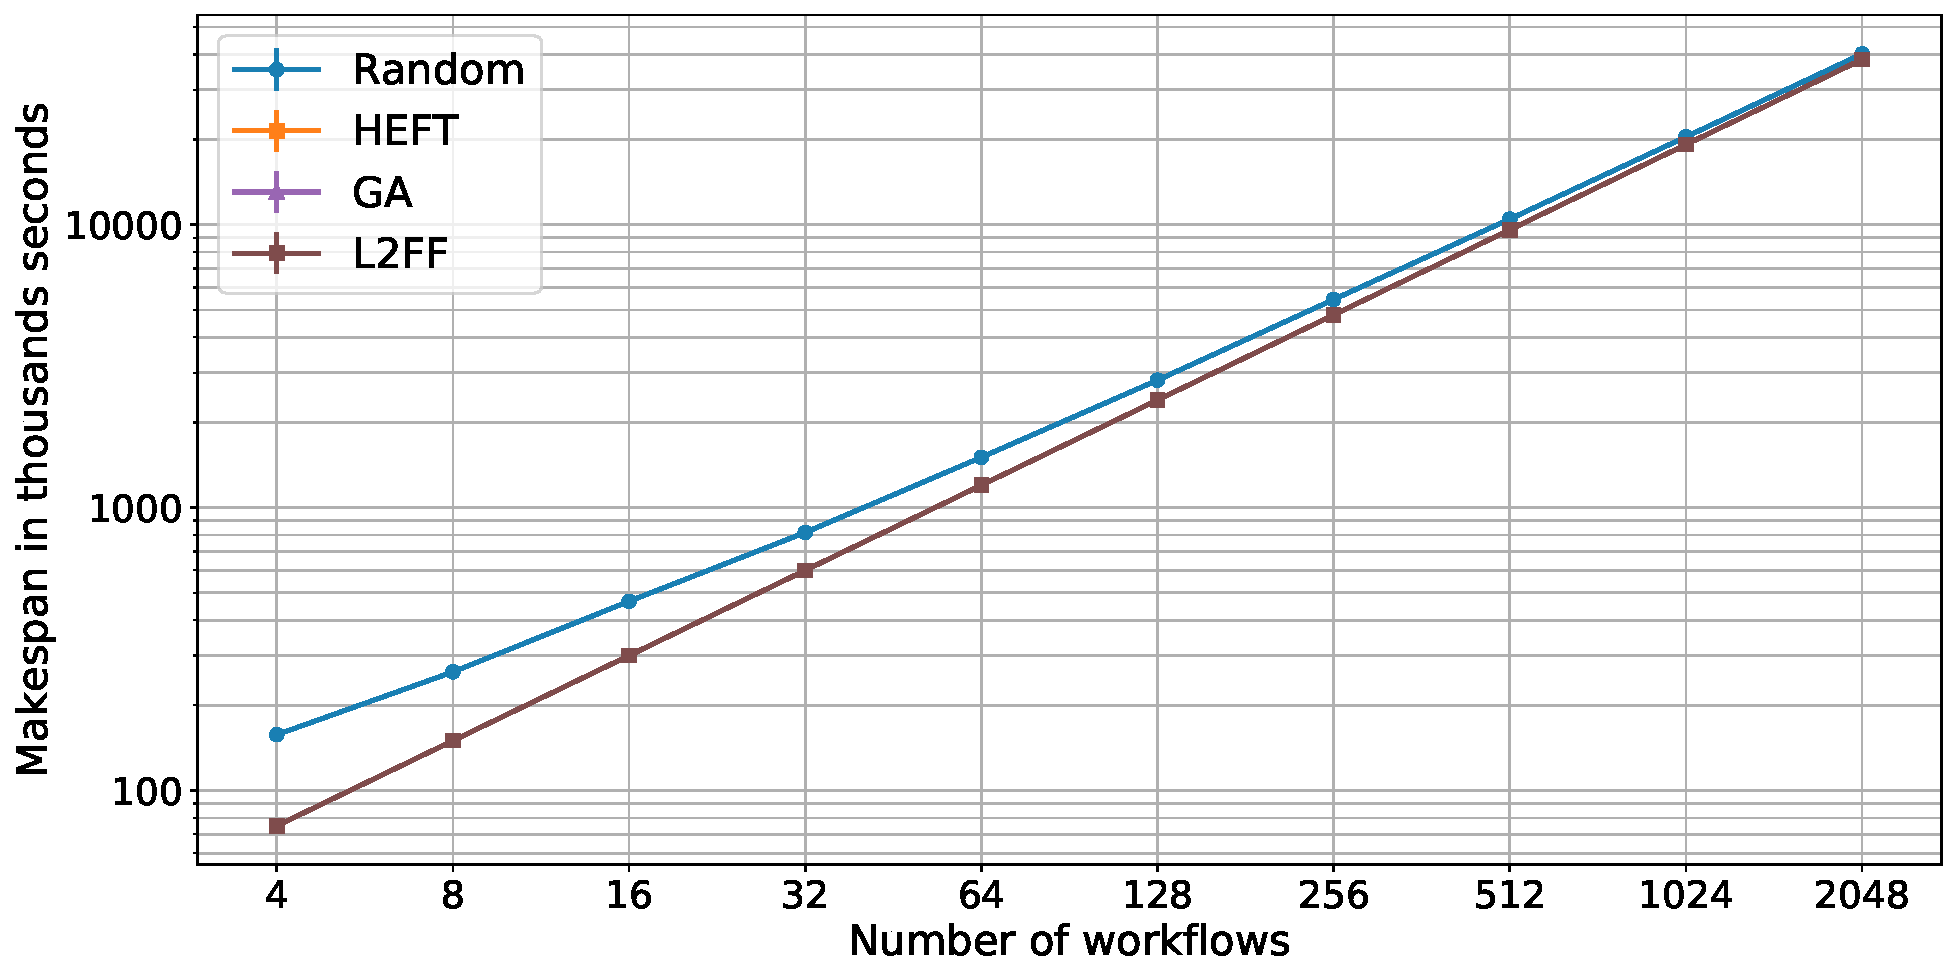
\includegraphics[width=.95\textwidth]{figures/campaign/StHomoCampaigns_4StHomoResources.pdf}
        \caption{}
        \label{fig:StHomoCampaigns_4StHomoResources}
    \end{subfigure}\\
    ~
    \begin{subfigure}[b]{0.75\textwidth}
        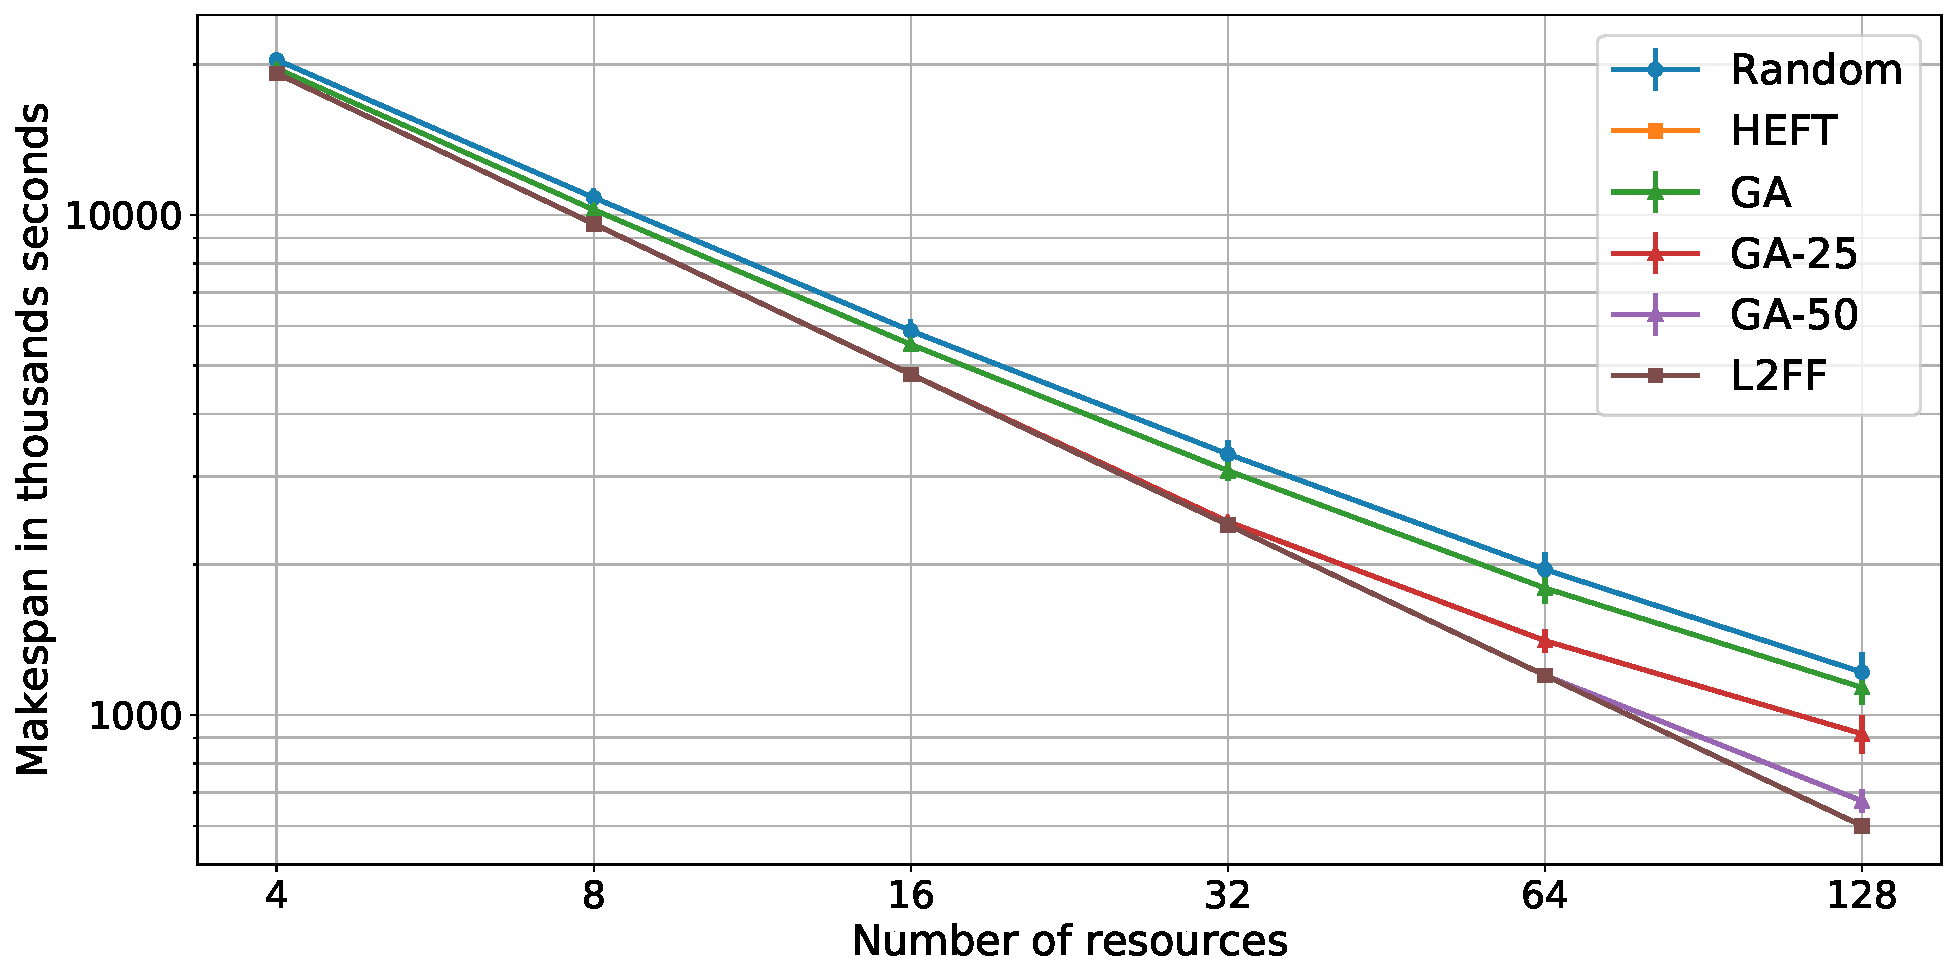
\includegraphics[width=.95\textwidth]{figures/campaign/StHomoResources_StHomoCampaigns.pdf}
        \caption{}
        \label{fig:StHomoResources_StHomoCampaigns}
    \end{subfigure}
    \caption{~\ref{fig:StHomoCampaigns_4StHomoResources} Makespan of increasing
    number of homogeneous workflows on homogeneous resources.
    \ref{fig:StHomoResources_StHomoCampaigns} Makespan of homogeneous campaign
    on different number of homogeneous resources.}
    \label{fig:st_homog_analysis}
\end{figure}

HEFT and L2FF provide better makespan than Random and GA. HEFT places a workflow
to the resource that will finish it earlier. L2FF places equal number of
workflows per resource for all available resources. As a result, both algorithms
are able to equally distribute the workflows to the resources. The genetic
algorithm shows worse makespan than HEFT and L2FF for more than 64 resources
(Fig.~\ref{fig:StHomoResources_StHomoCampaigns}), verifying our expectation
based on its convergence rate.

%\subsubsection*{Heterogeneous Campaign -- Heterogeneous Resources}
%The next configuration of this experiment shows how resource heterogeneity affects the performance of the algorithms.
%The three selected algorithms produce and use different information about resources and specifically resource availability.
%HEFT and GA-50 estimate when a resource is available and L2FF uses the number of workflows on a resource as resource availability.
%Based on the information they produce, we expect the algorithms that produce more exact information to have better performance, such as HEFT and GA-50.

%\begin{figure*}[ht!]
%    \centering
%    \begin{subfigure}[b]{0.75\textwidth}
%        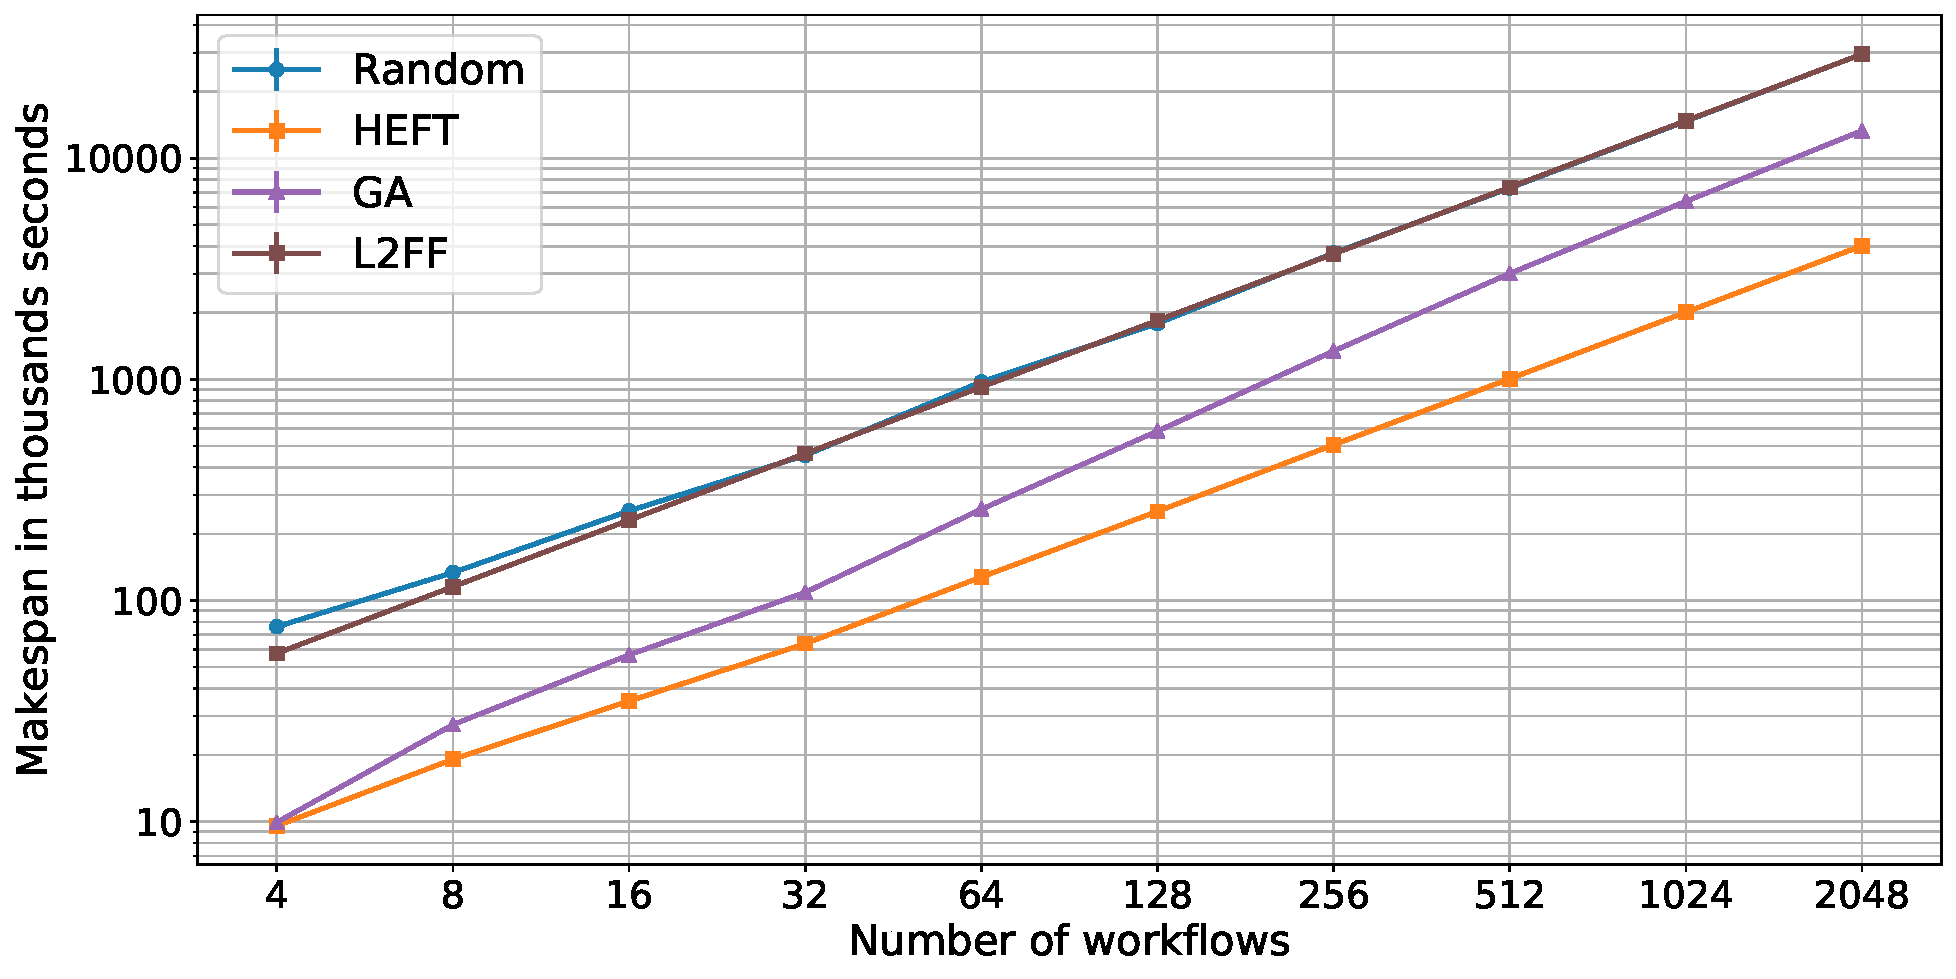
\includegraphics[width=.95\textwidth]{figures/campaign/StHomoCampaigns_4StHeteroResources.pdf}
%        \caption{}
%        \label{fig:StHomoCampaigns_4StHeteroResources}
%    \end{subfigure}\\
%    ~
%    \begin{subfigure}[b]{0.75\textwidth}
%        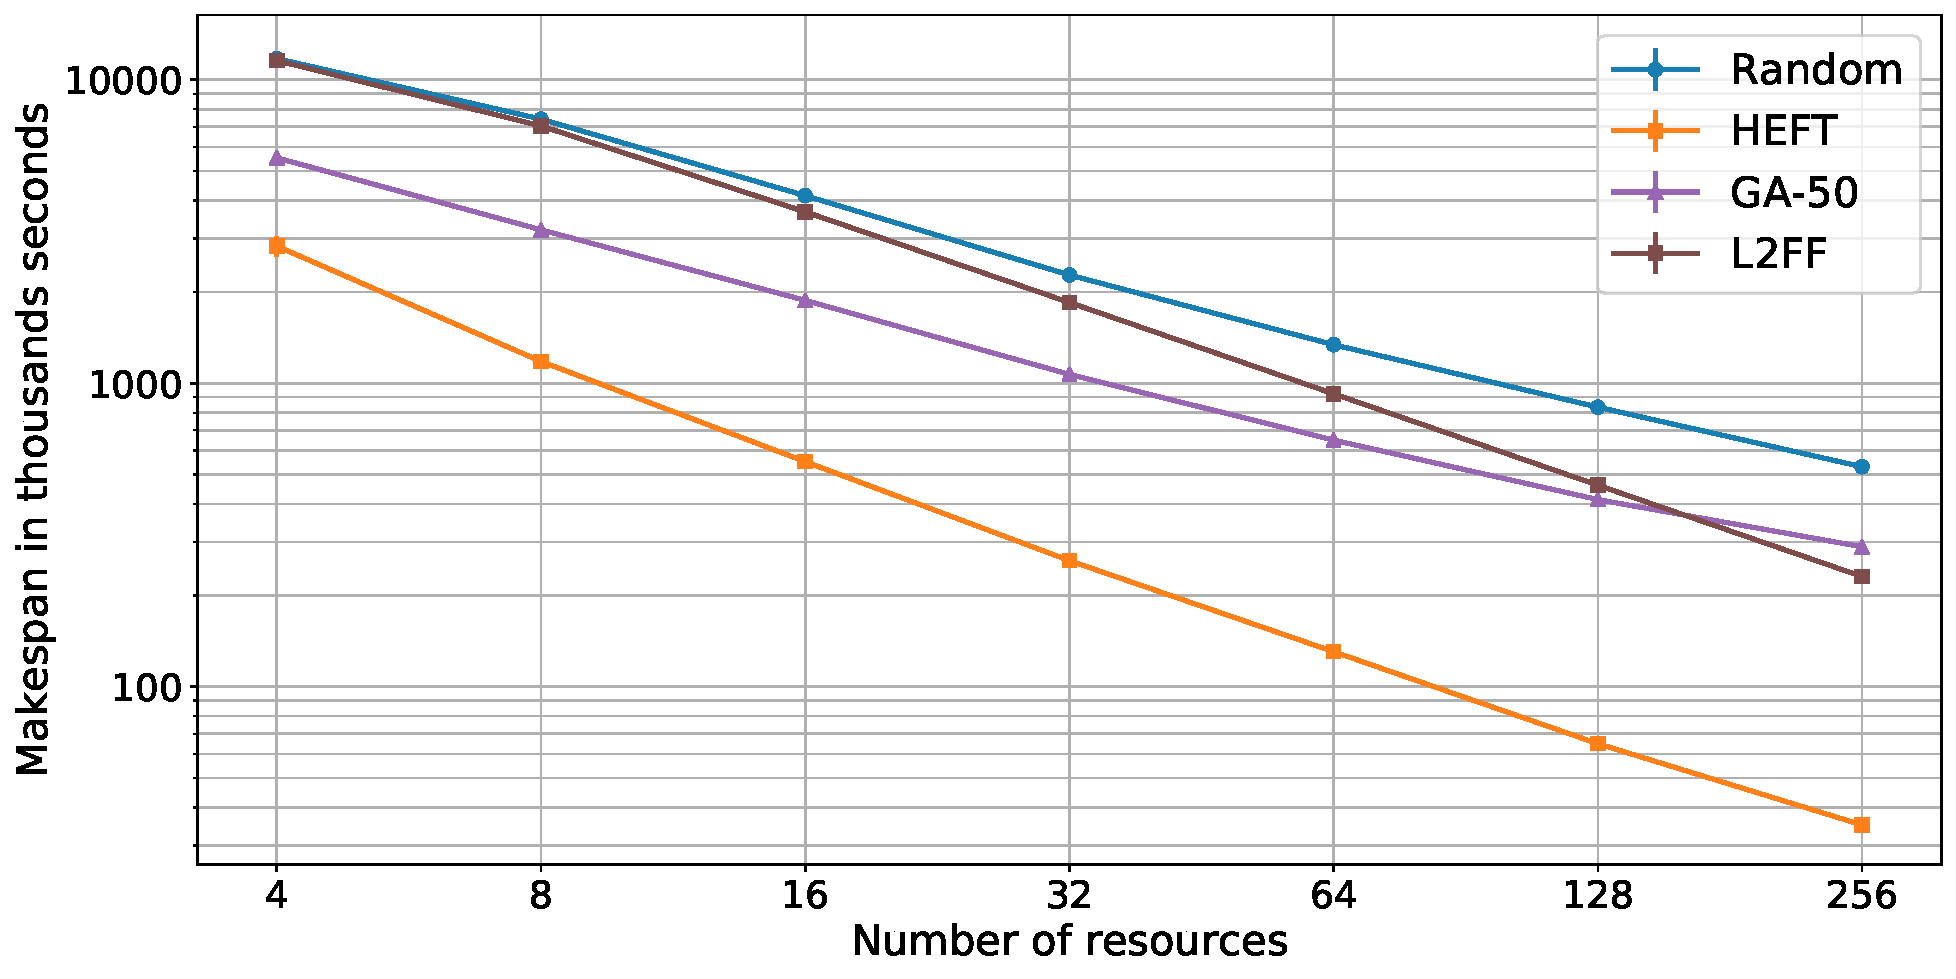
\includegraphics[width=.95\textwidth]{figures/campaign/StHeteroResources_StHomoCampaigns.pdf}
%        \caption{}
%        \label{fig:HeteroResources_StHomoCampaigns}
%    \end{subfigure}
%    \caption{Makespan of homogeneous workflows on heterogeneous resources:~\ref{fig:StHomoCampaigns_4StHeteroResources}) varying campaign size with 4 resources;
%        ~\ref{fig:HeteroResources_StHomoCampaigns}) varying number of resources for constant campaign size at 1024 workflows.}
%    \label{fig:hom_het_analysis}
%\end{figure*}

Figure~\ref{fig:heter_analysis} shows the makespan of the three algorithms for
a campaign with heterogeneous workflows on heterogeneous resources. Workflows
are heterogeneous when they have different runtime and resources are
heterogeneous when they have different performance. Specifically, workflow
runtimes are drawn randomly from a normal distribution with mean of 75000
seconds and variance of 6000 seconds. Heterogeneous resources are drawn
randomly from the four resources described before.

HEFT provides up to an order of magnitude better makespan than L2FF and GA
whether the campaign size (Fig.~\ref{fig:StHeteroCampaigns_4StHeteroResources})
or the number of resources (Fig.~\ref{fig:StHeteroResources_StHeteroCampaigns})
changes. In addition, GA produces plans with at least two times better makespan
that L2FF when resources are constant and the number of workflows changes. As
the number of resources increase, the difference between the plans that GA and
L2FF produce reduces with L2FF providing a plan with better makespan than GA for
256 resources. For up to 64 resources, the heuristic of GA based on earlier
finish time, reduces the effect of random initialization. This is not the
case for 128 and 256 resources though, as the random part of the initialization
may place very few or no workflows on some resources. L2FF places the same
number of workflows per resource and, as a result, overutilizes less performant
resources. HEFT instead ranks the workflows and places each workflow on the
resource that will finish it earlier. As a result, HEFT tries to place each
workflow on the resource that causes the minimum makespan increase for the given
set of resources.

\begin{figure*}[t]
    \centering
    \begin{subfigure}[b]{0.75\textwidth}
        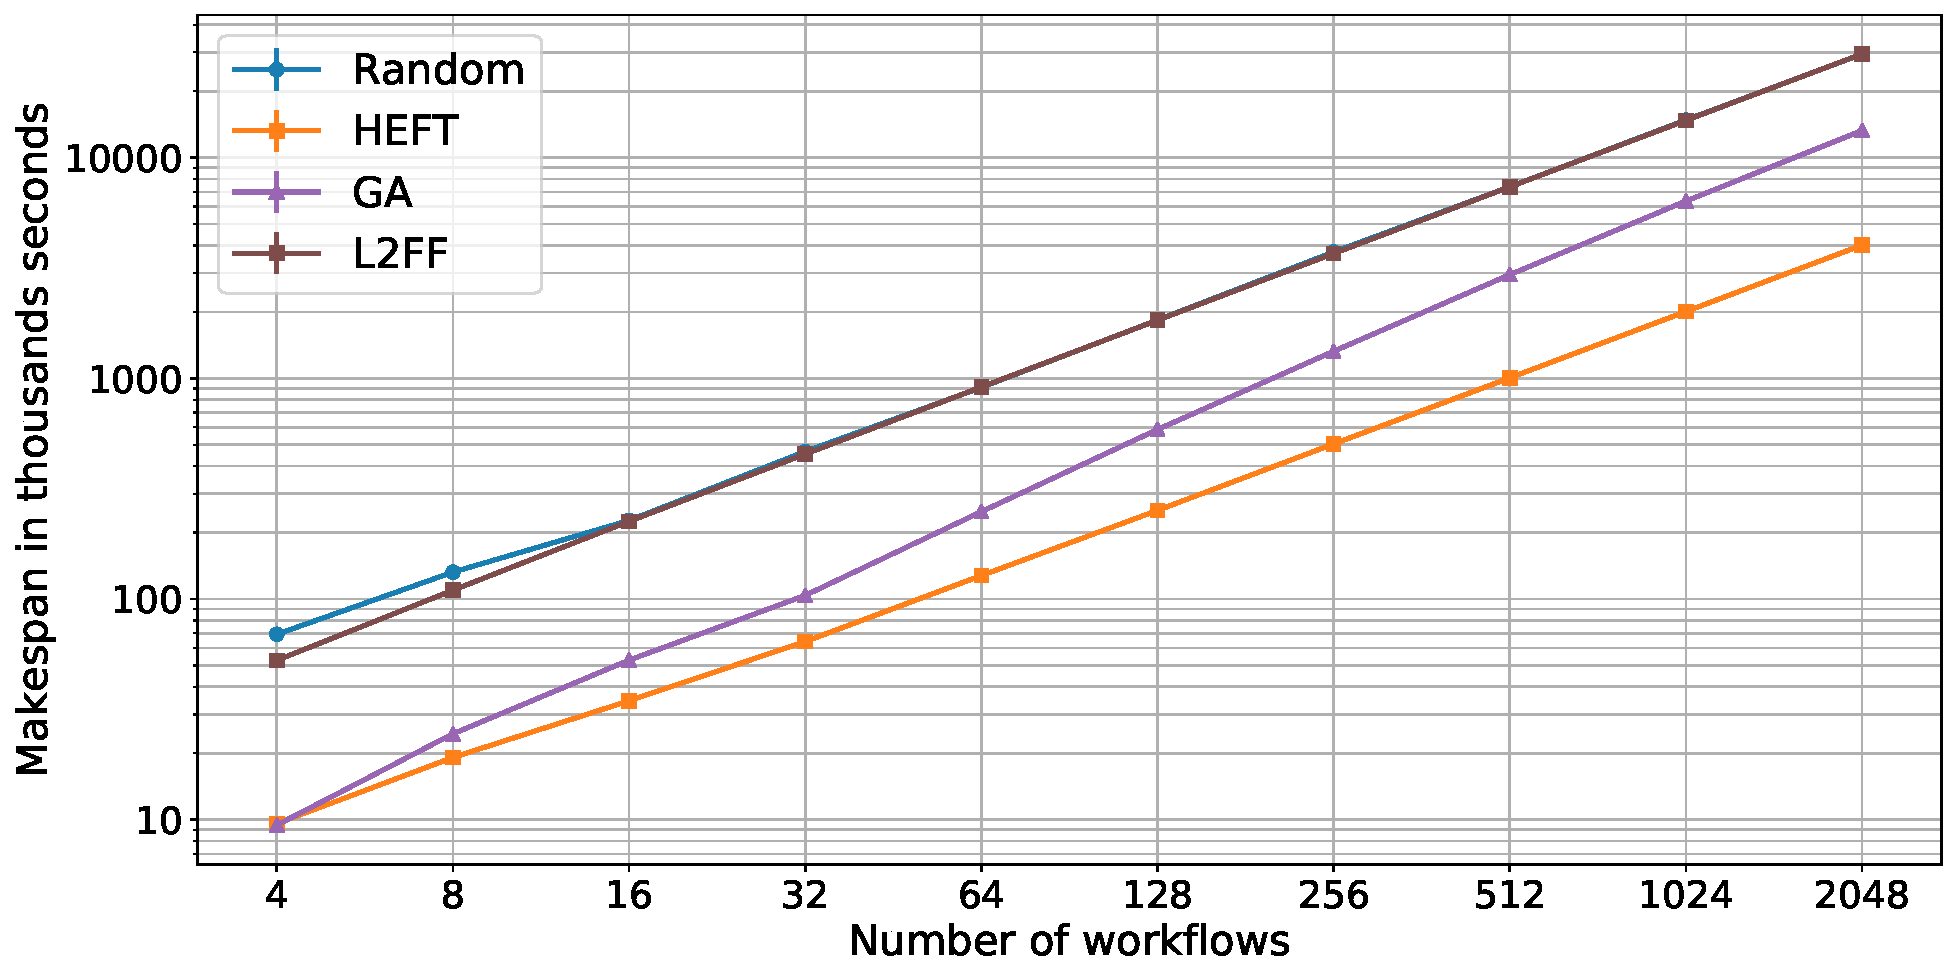
\includegraphics[width=.95\textwidth]{figures/campaign/StHeteroCampaigns_4StHeteroResources.pdf}
        \caption{}
        \label{fig:StHeteroCampaigns_4StHeteroResources}
    \end{subfigure}\\
    ~
    \begin{subfigure}[b]{0.75\textwidth}
        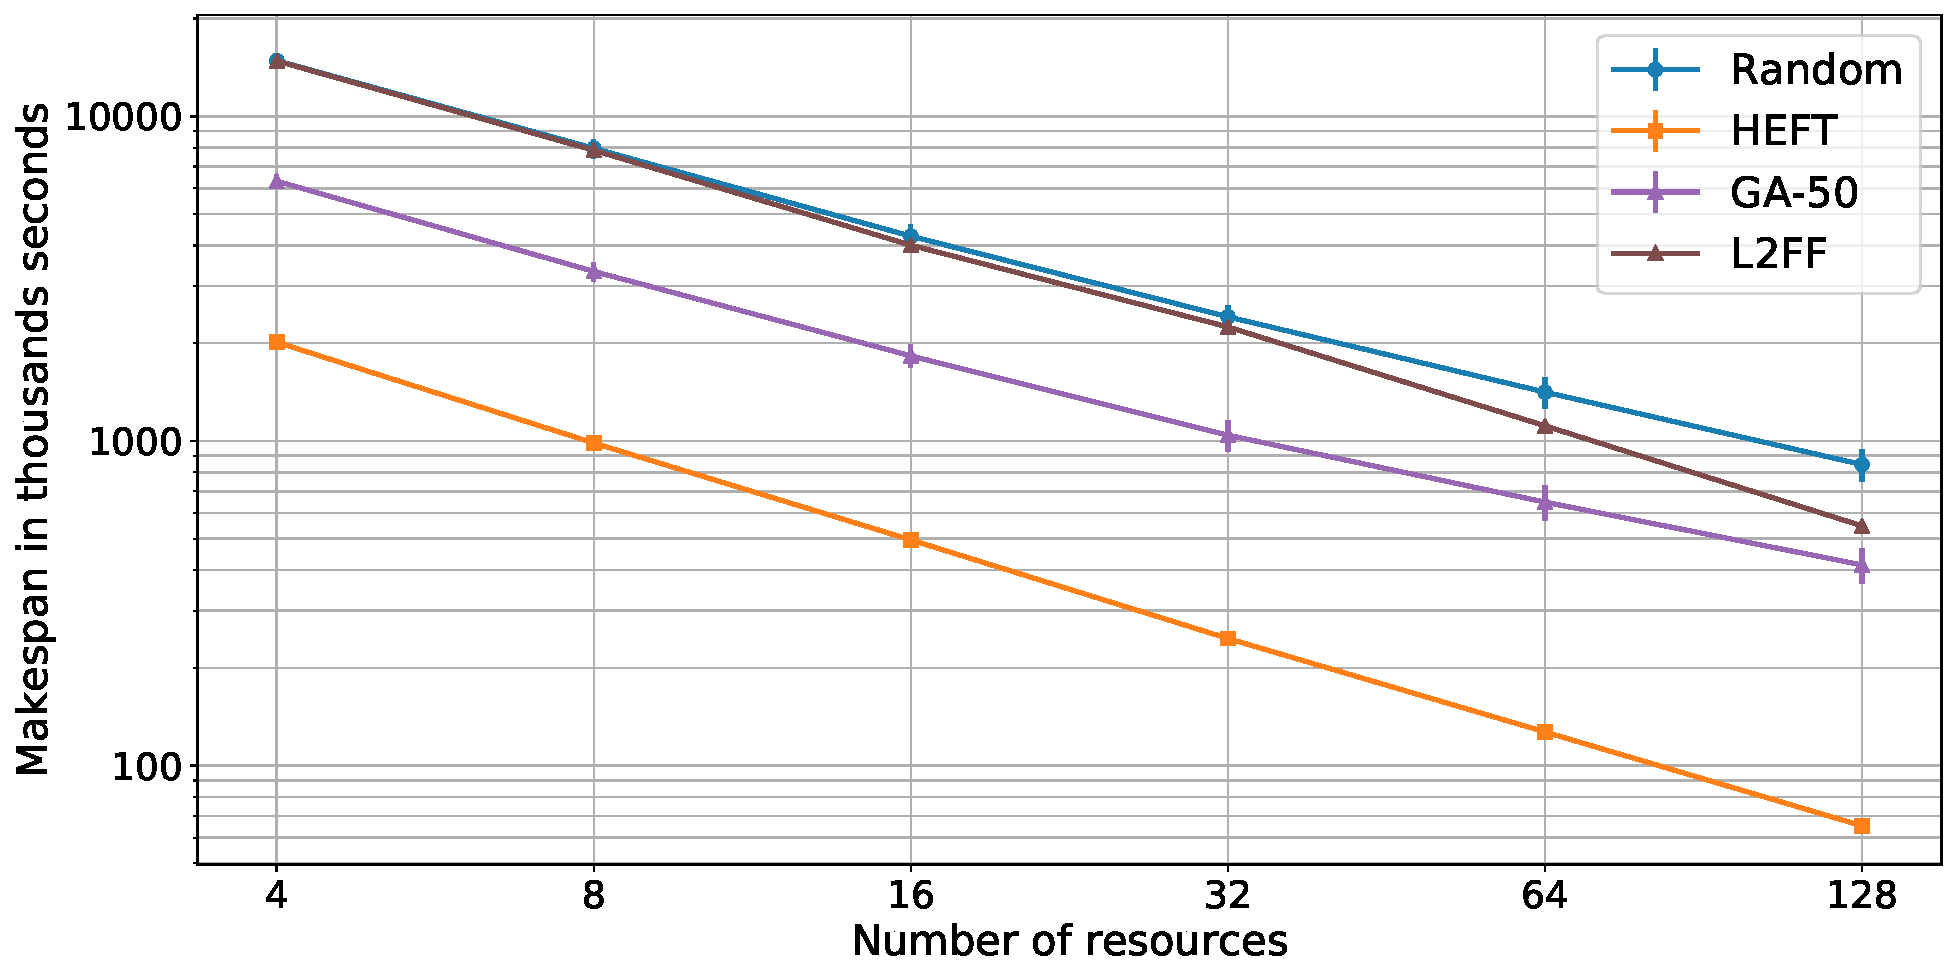
\includegraphics[width=.95\textwidth]{figures/campaign/StHeteroResources_StHeteroCampaigns.pdf}
        \caption{}
        \label{fig:StHeteroResources_StHeteroCampaigns}
    \end{subfigure}
    \caption{~\ref{fig:StHeteroCampaigns_4StHeteroResources}) Makespan of 4 up
        to 2048 heterogeneous workflows on 4 heterogeneous resources;
        \ref{fig:StHeteroResources_StHeteroCampaigns}) Makespan of a
        heterogeneous campaign with 1024 workflows on different 4 up to 256
        heterogeneous resources.}
    \label{fig:heter_analysis}
\end{figure*}

In summary, we conclude that resource heterogeneity dominates the makespan
performance among the considered algorithms. On homogeneous resources, HEFT,
GA and L2FF plans produce plans with similar makespan to each other. On
heterogeneous resources, HEFT makespan is at least an order of magnitude
smaller than L2FF makespan and is more than two times smaller than GA makespan
independent of workflow homogeneity or heterogeneity.

A common characteristic between HEFT and GA is that they create an expectation
of when resources will be available, in contrast to L2FF which considers a
resource available based on the number of workflows.
% As a result, the resource availability expectation is the dominant
% characteristic among the three algorithms.
Further, HEFT is deterministic, while GA is not, and HEFT always performed
better than GA.
% Thus, the second characteristic that affect the makespan is whether an
% algorithm is deterministic or not.
Thus, the characteristics of the selected algorithms that affect the
makespan performance, in order of importance, are:
\begin{inparaenum}[(1)]
    \item estimating when a resource will be available;
    \item deterministic or randomized heuristics; and
    \item creating a workflow priority list based on workflow runtime
\end{inparaenum}

\subsection{Experiment 2: Sensitivity of Makespan to Resource Dynamism}

High performance computing (HPC) resources show performance variations for
multiple reasons, including power constrained
operations~\cite{inadomi2015analyzing}, network and shared filesystem
congestion~\cite{brown2018interference} and performance
degradation~\cite{wu2017survey}. Following established literature, the rate at
which the performance of a resource changes is days to
years~\cite{skinner2005understanding}. Thus, we model resource dynamism as the
daily change in the performance of a resource. We draw the performance values
from a normal distribution, with a mean value equal to the performance of that
resource and sigma to 6~\% of the mean \mtnote{Why 6\%}.
Figure~\ref{fig:dynamic_res} shows the histogram of a dynamic resource
performance with a mean value of 1 petaFLOP.

\begin{figure}[t]
    \centering
    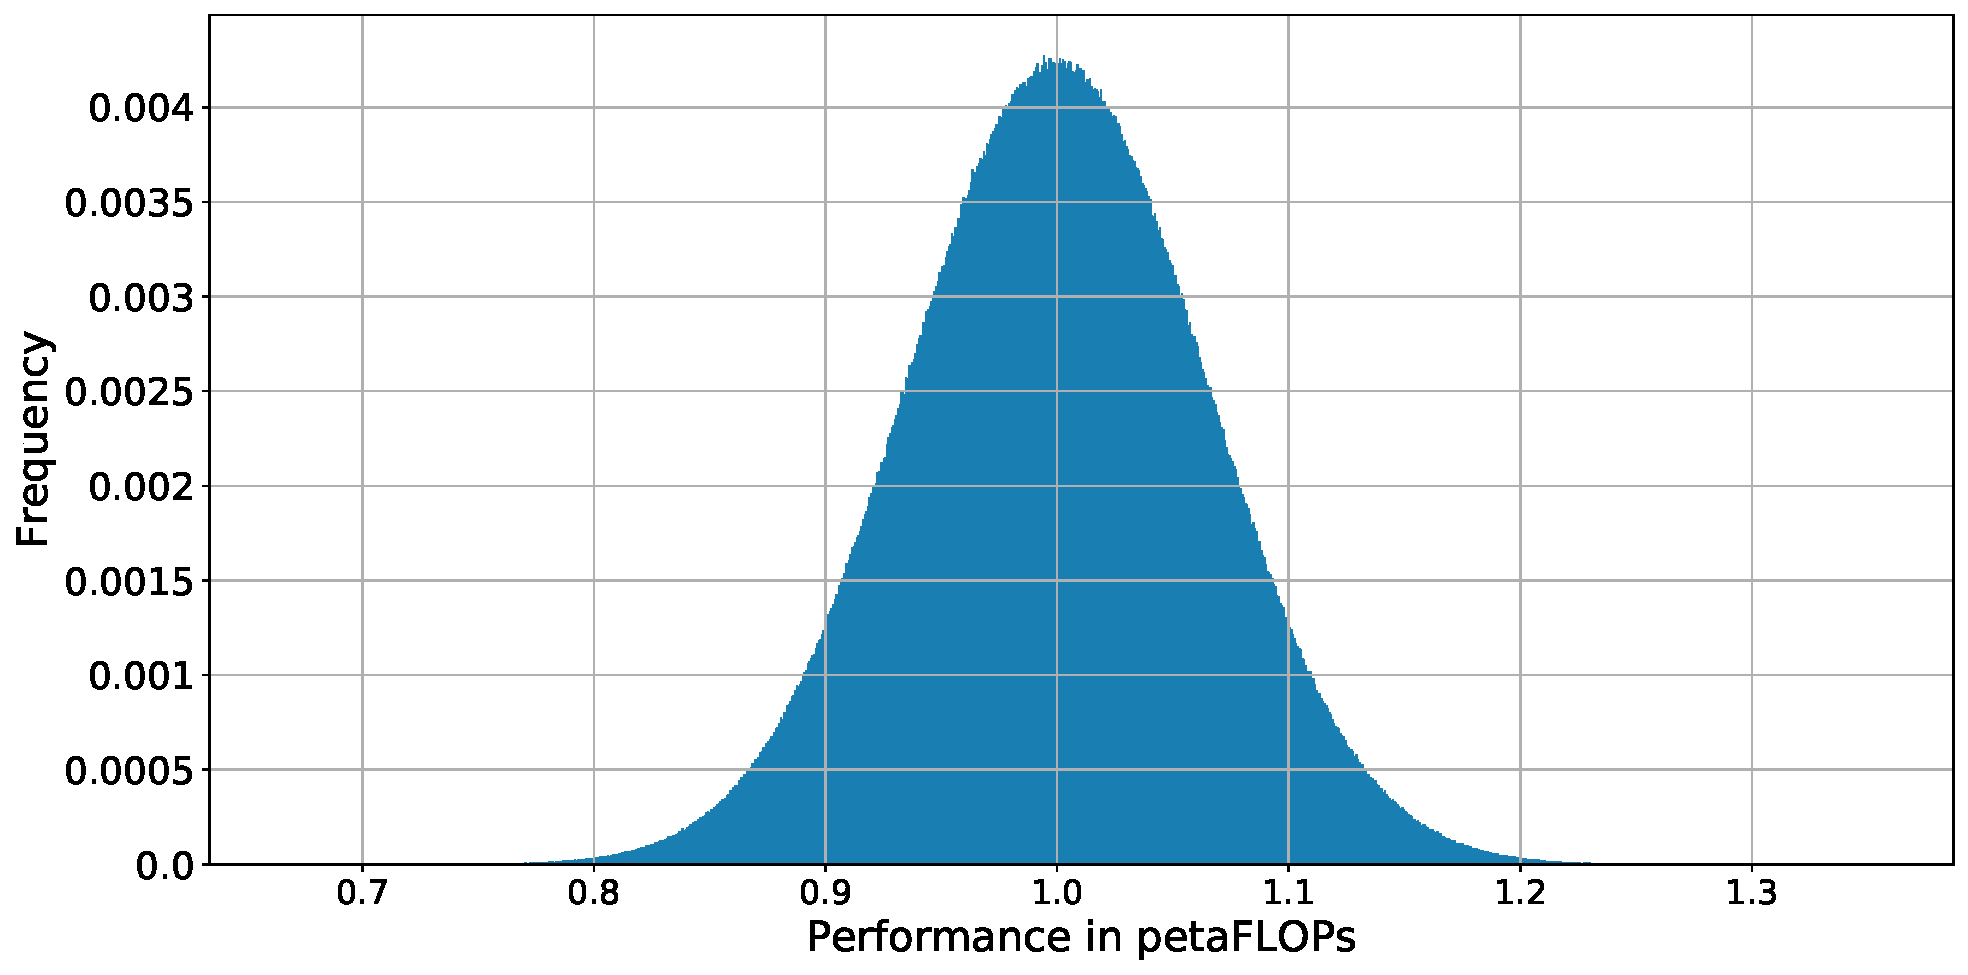
\includegraphics[width=.75\textwidth]{figures/campaign/DynRes.pdf}
    \caption{Resource performance distribution of a dynamic resource with 1
    petaFLOP average performance.}
    \label{fig:dynamic_res}
\end{figure}

In experiment 2, we measure the sensitivity of the makespan using HEFT, L2FF, GA
and Random to resource dynamism on homogeneous and heterogeneous resources. We
define makespan sensitivity $Sens$ as the difference between the makespan
measured via executing a campaign, $TTX_{C, Exec}$, and the expected makespan
given by the execution plan, $TTX_{C}(M)$, thus $Sens = TTX_{C, Exec} -
TTX_{C}(M)$. Based on the results of experiment 1, we expect $Sens$ to be
similar between algorithms on homogeneous resources, as the three algorithms
produce similar plans. On heterogeneous resources, we expect HEFT and L2FF to
show higher sensitivity than GA and Random, as GA and Random may produce a plan
that does not utilize a resource which performance results to be significantly
slower than expected at runtime. Figures~\ref{fig:dyn_homog_sens_analysis}
and~\ref{fig:dyn_hetero_sens_analysis} show the results for homogeneous
workflows and homogeneous resources, and for heterogeneous workflows and
heterogeneous resources respectively.

\begin{figure}[ht!]
    \centering
    \begin{subfigure}[b]{0.75\textwidth}
        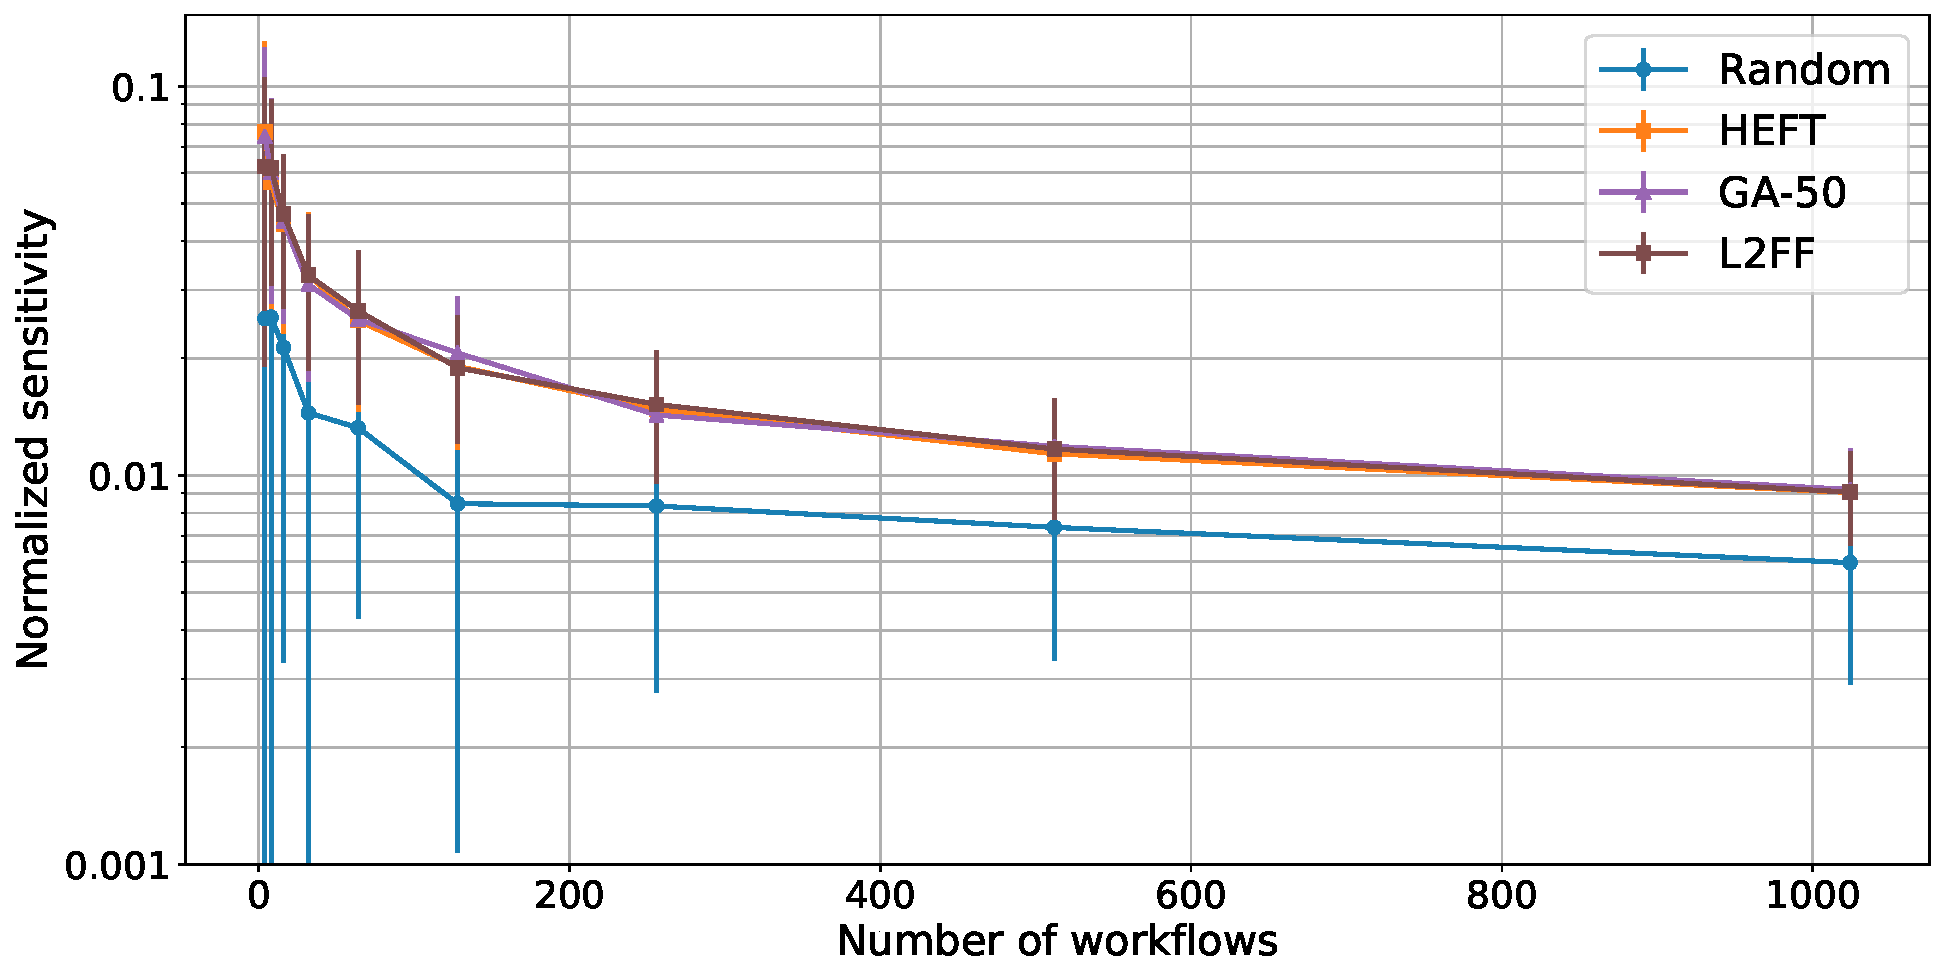
\includegraphics[width=.95\textwidth]{figures/campaign/StHomoCampaigns_4DynHomoResourcesSens.pdf}
        \caption{}
        \label{fig:StHomoCampaigns_4DyHomoResourcesSens}
    \end{subfigure}\\
    ~
    \begin{subfigure}[b]{0.75\textwidth}
        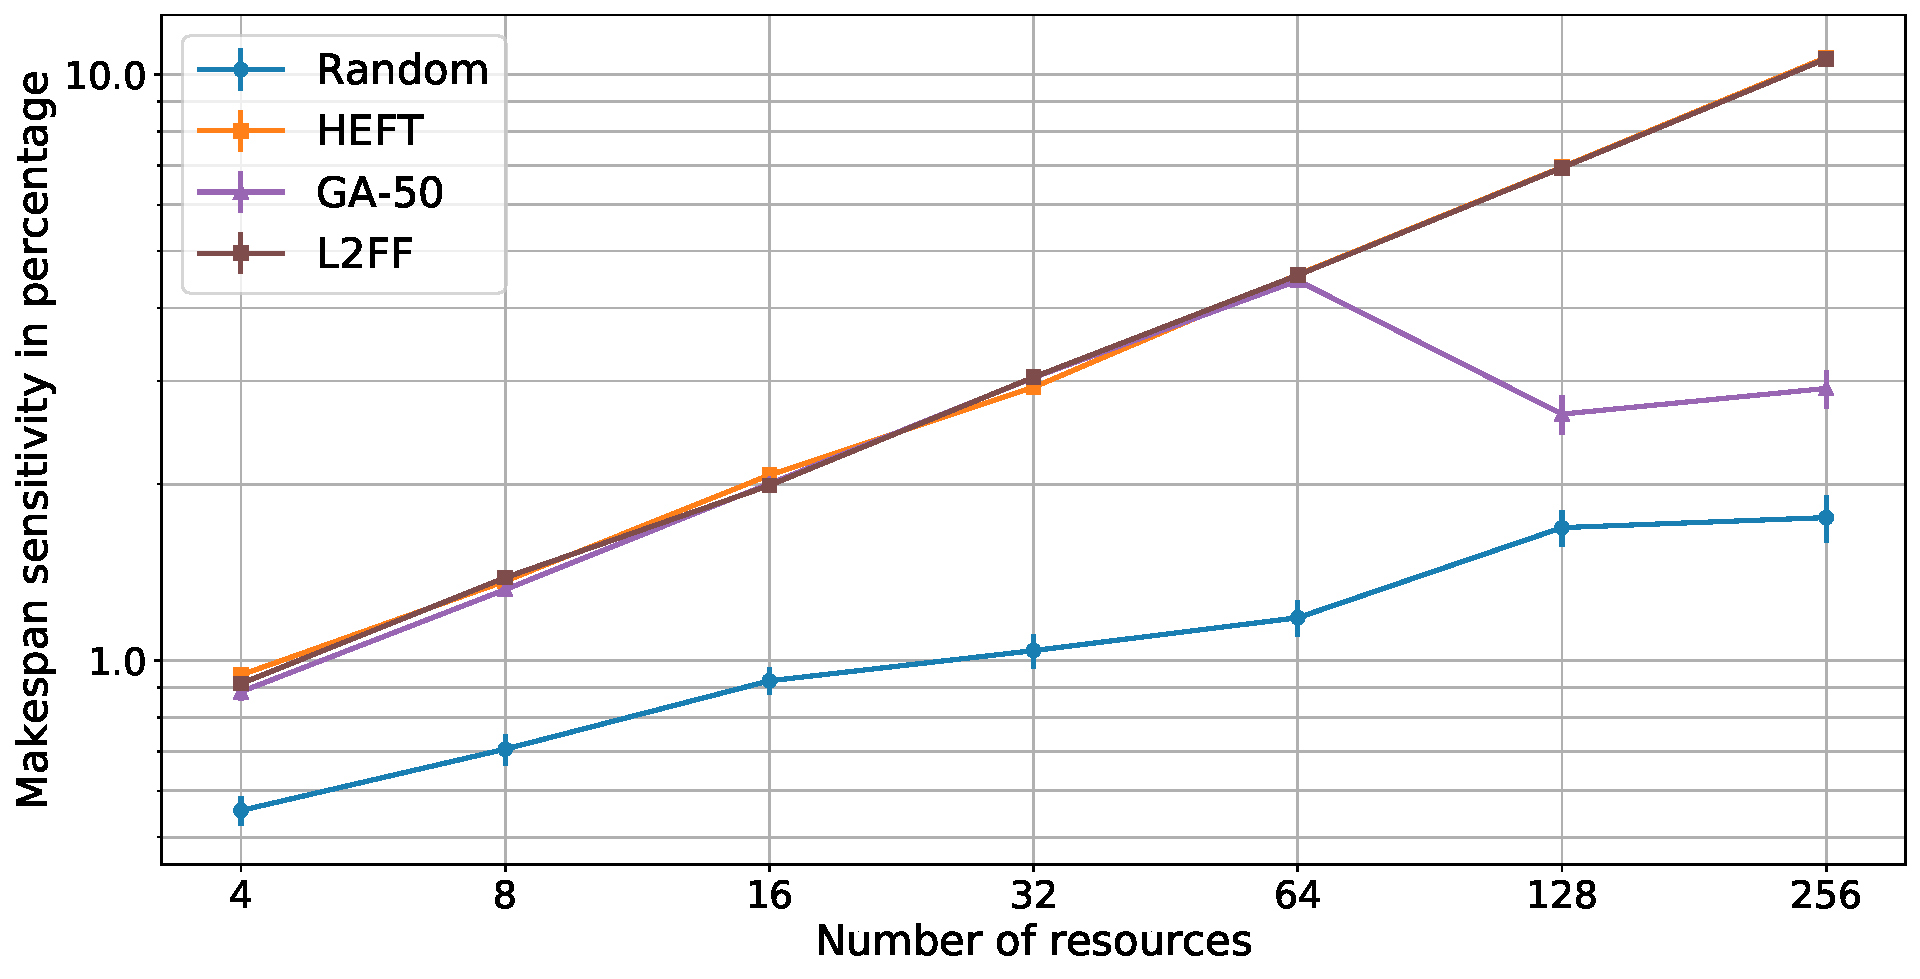
\includegraphics[width=0.95\textwidth]{figures/campaign/DynHomoResources_StHomoCampaignsSens.pdf}
        \caption{}
        \label{fig:DyHomoResources_StHomoCampaignsSens}
    \end{subfigure}
    \caption{Sensitivity of makespan in percentage of homogeneous workflows on
        homogeneous resources. \ref{fig:StHomoCampaigns_4DyHomoResourcesSens}
        increasing number of workflows and 4 resources;
        \ref{fig:DyHomoResources_StHomoCampaignsSens} 1024 workflows and
        increasing number of resources.}
    \label{fig:dyn_homog_sens_analysis}
\end{figure}

As per our expectation, the sensitivity of makespan among the three algorithms
is similar and it is between 1~\% and 10~\% (see
Fig.~\ref{fig:StHomoCampaigns_4DyHomoResourcesSens}
and~\ref{fig:DyHomoResources_StHomoCampaignsSens}). In addition, we observe a
drop in GA sensitivity at 128 resources. GA produces different plans at every
realization of the experiment, since it places a number of workflows to
resources randomly and, as a result, some plans are affected less from resource
dynamism. In addition, sensitivity drops as the number of workflows increases
and the number of resources is constant
(Fig.~\ref{fig:StHomoCampaigns_4DyHomoResourcesSens}). Sensitivity increases
when the number of resources increases and the number of workflows is constant
(Fig.~\ref{fig:DyHomoResources_StHomoCampaignsSens}). Thus, the sensitivity
decreases when the average number of workflows per resource increases,
regardless for how workflows are placed onto resource by a plan.

Figure~\ref{fig:dyn_hetero_sens_analysis} shows the makespan sensitivity as a
percentage for a campaign of heterogeneous workflows and heterogeneous
resources. Makespan sensitivity shows similar values---from 3\% to $<1$\%---for
all three algorithms in
figure~\ref{fig:StHeteroCampaigns_4DyHeteroResourcesSens}, except for HEFT with
more than 512 workflows contrary to our expectation. We explain this behavior by
noticing that, as more workflows are placed on each resource, it becomes more
probable that the effect of a potential slowdown of a workflow is reduced. This
is because some workflows will finish faster and therefore reduce the
sensitivity of the plan.

Figure~\ref{fig:DyHeteroResources_StHeteroCampaignsSens} shows different
sensitivity values for each algorithm. HEFT is at least two times more sensitive
than GA and L2FF. HEFT places workflows on resources so that all resources are
used for the least possible amount of time. As a result, a slow down on a
resource will affect the makespan with HEFT more than that with GA and L2FF,
which produce plans that overutilize some resources. Further, the sensitivity
values for all algorithms are significantly lower than those observed when
homogeneous resources were used, as a potential slowdown on a performant
resource will not significantly affect the makespan of the campaign. In
addition, we see that: (1) makespan sensitivity decreases as the number of
workflows increases; and (2) makespan sensitivity increases as the number of
resources increases. This further supports our conclusion that makespan
sensitivity decreases as the average number of workflows per resource increases.

Based on the results in
figure~\ref{fig:DyHeteroResources_StHeteroCampaignsSens}, we see that the
number of resources is a more dominant factor than resource heterogeneity for
makespan sensitivity. HEFT-based plans are more sensitive that GA, L2FF and
Random up to 64 resources. L2FF becomes more sensitive for more than 128
resources and is more sensitive to changes on less performant resources.

\begin{figure}[ht!]
    \centering
    \begin{subfigure}[b]{0.85\textwidth}
        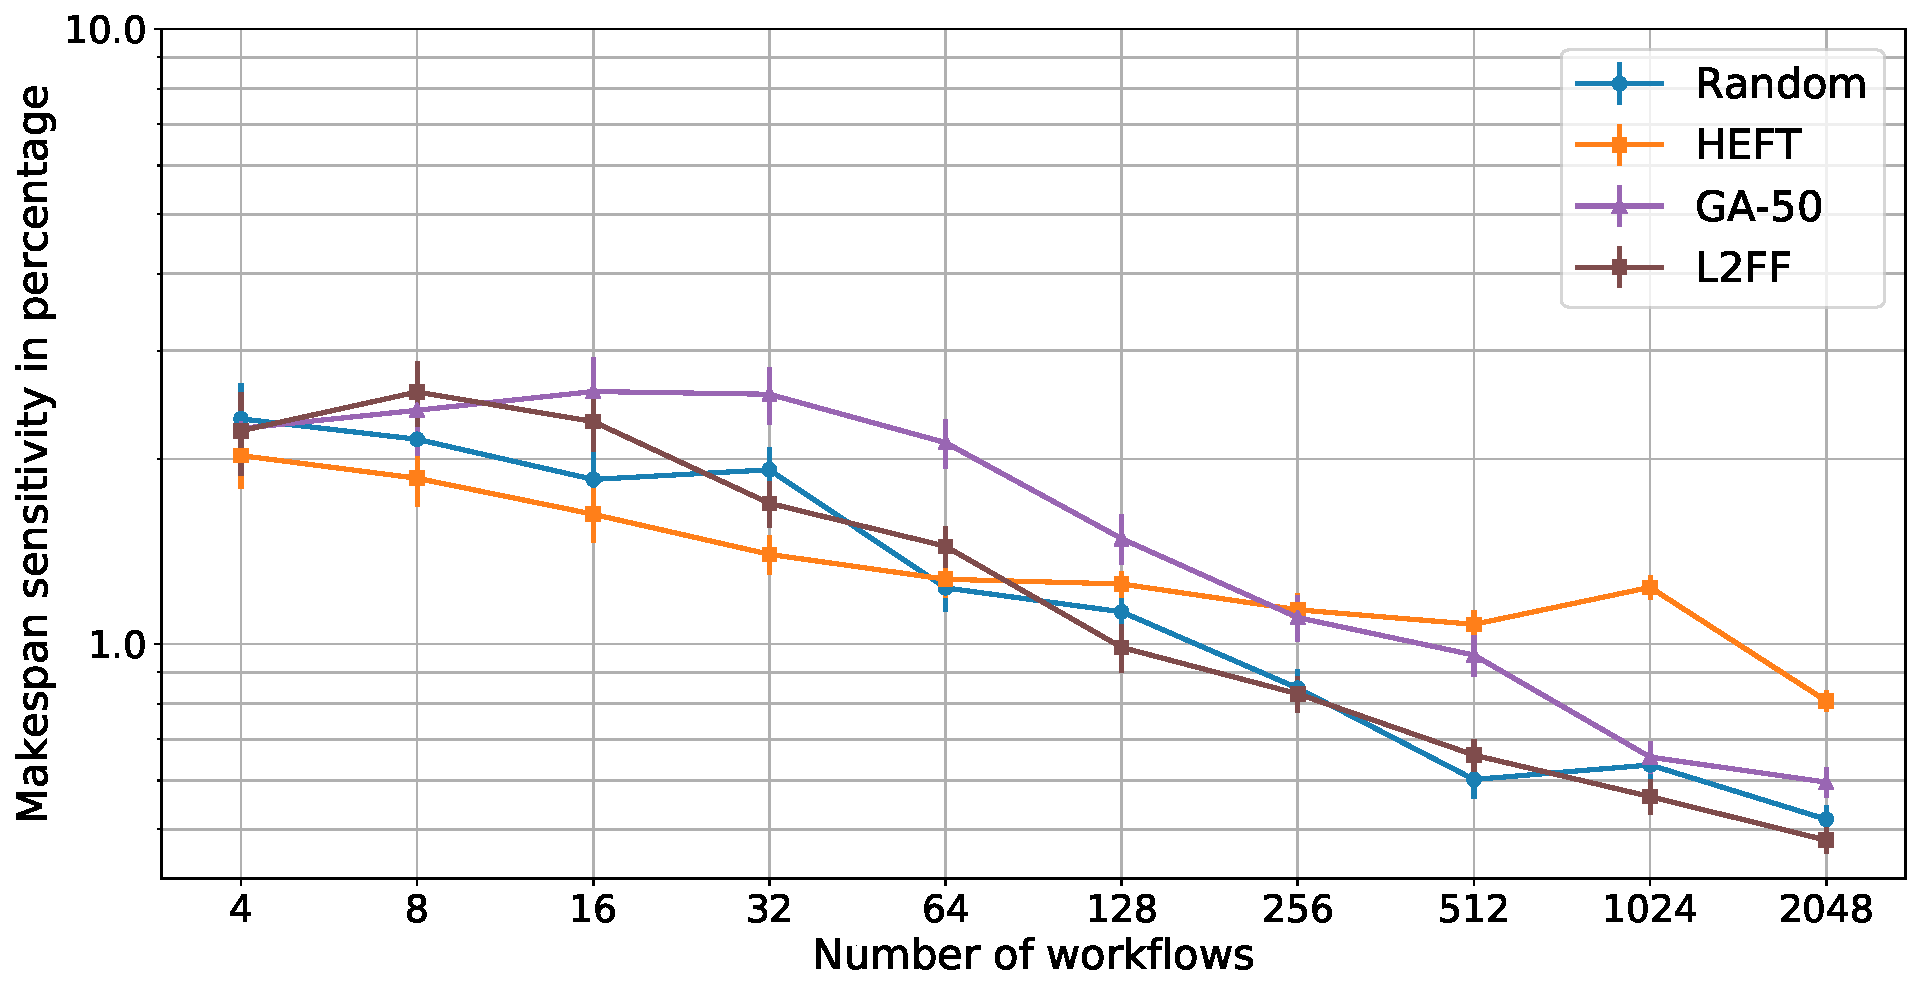
\includegraphics[width=.95\textwidth]{figures/campaign/StHeteroCampaigns_4DynHeteroResourcesSens.pdf}
        \caption{}
        \label{fig:StHeteroCampaigns_4DyHeteroResourcesSens}
    \end{subfigure}\\
    ~
    \begin{subfigure}[b]{0.85\textwidth}
        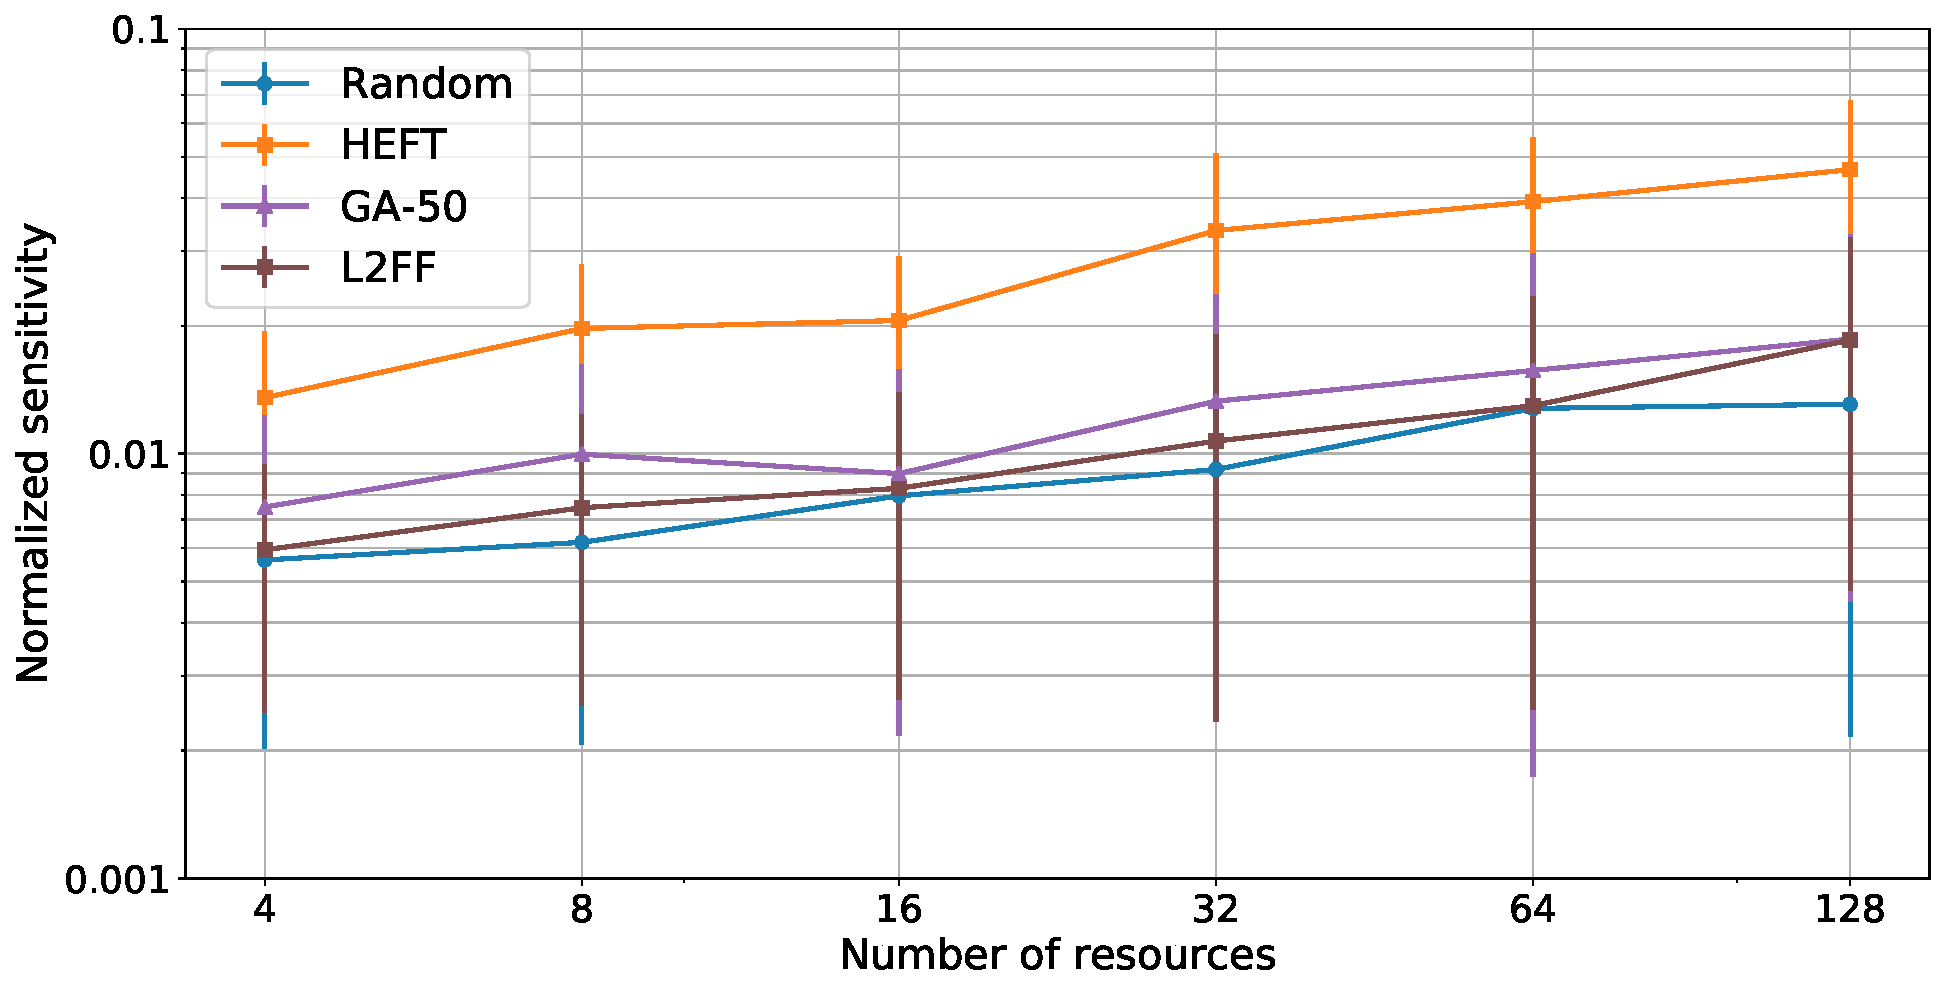
\includegraphics[width=0.95\textwidth]{figures/campaign/DynHeteroResources_StHeteroCampaignsSens.pdf}
        \caption{}
        \label{fig:DyHeteroResources_StHeteroCampaignsSens}
    \end{subfigure}
    \caption{Sensitivity of makespan in percentage of heterogeneous workflows on
    heterogeneous resources. \ref{fig:StHeteroCampaigns_4DyHeteroResourcesSens}
    increasing number of workflows and 4 resources;
    \ref{fig:DyHeteroResources_StHeteroCampaignsSens} 1024 workflows and
    increasing number of resources.}
    \label{fig:dyn_hetero_sens_analysis}
\end{figure}

Experiment 2 measured how sensitive plans are when using HEFT, GA, L2FF and
Random in presence of resource dynamism. On homogeneous resources, all
algorithms show similar levels of sensitivity. GA sensitivity drops from more
than 64 resources as some resources are overutilized. On heterogeneous
resources, HEFT is generally more sensitive as it tries to place a workflow to a
resource with the least impact on the campaign makespan. L2FF becomes more
sensitive than HEFT after 128 resources as it places equal number of workflows
to resources, progressively overutilizing less performant resources. In
addition, sensitivity is proportional to the number of resources and inverse
proportional to the number of workflows, since it decreases as the number of
workflows increases when using constant number of resources and increases when
number of resources increases and campaign size is constant. Finally, we
observed that a 6~\% performance variation in the resources causes less than
10~\% variation in makespan, regardless if resources are homogeneous or
heterogeneous.

\subsection{Experiment 3: Sensitivity of Makespan to Workflow Runtime Estimation Uncertainty}

All selected algorithms, HEFT, GA and L2FF, require an estimation about the
runtime of each workflow of the campaign. Users usually derive this information
from empirical data, creating uncertainty in the workflow runtime estimation.
This uncertainty has the potential to affect the makespan of the campaign, as
the runtime estimation is used to either derive information about workflows
runtime on resources (HEFT and GA) or rank workflows (L2FF). Similarly to
experiment 2, we want to understand how different levels of uncertainty affect
the makespan of the plans produced by HEFT, GA and L2FF

We introduce workflow runtime estimation uncertainty as the difference between
the estimated and actual runtime of a workflow on a 1 petaFLOP resource.
Specifically, we denote as $u$ the level of uncertainty between $[0,1]$, $u'$
the uncertainty for a workflow drawn randomly from the range $[-u,u]$, and
$Tx_{w}$ the mean estimated runtime of a workflow. Thus, the actual runtime of
a workflow is $ Tx_{w'} = Tx_{w} \times (1-u')$.

In experiment 3, we measure the sensitivity of makespan, as defined in
experiment 2, to workflow runtime estimation uncertainty for level of
uncertainty from 10~\% to 50~\%. As all algorithms produce similar plans on
homogeneous resources, exposing the plans to the same variation should show the
same effect, regardless of the used algorithm. This is supported by the fact
that we measure the sensitivity after the execution of a campaign, and compare
it to the expected makespan produced by the plan. Accordingly, we limit
experiment 3 onlt to heterogeneous workflows executing on heterogeneous
resources.

We expect sensitivity to workflow runtime estimation uncertainty to decrease as
the number of workflows increases, and to increase as the number of resources
decreases. As the number of workflows increases, more workflows are placed on a
resource. As a result, on one hand it is more probable that a potential increase of
the makespan due to a longer than expected workflow is hidden
by other workflows than are shorter than expected. On the other hand, as the
number of resources increases, fewer workflows are placed on each resource and a
potentially larger workflow will have significant impact on the overall
makespan. This is especially true when heterogeneous resources are used and a
long workflow is placed on a less performant resource.
Figure~\ref{fig:inaccur_st} shows the results of experiment 3 with varying
number of workflows (figure~\ref{fig:InaccurStHeteroCampaigns_4StHeteroResourcesSens}) and
varying number of resources (\ref{fig:InaccurStHeteroResources_StHeteroCampaignsSens}).

\begin{figure}[ht!]
    \centering
    \begin{subfigure}[b]{0.95\textwidth}
        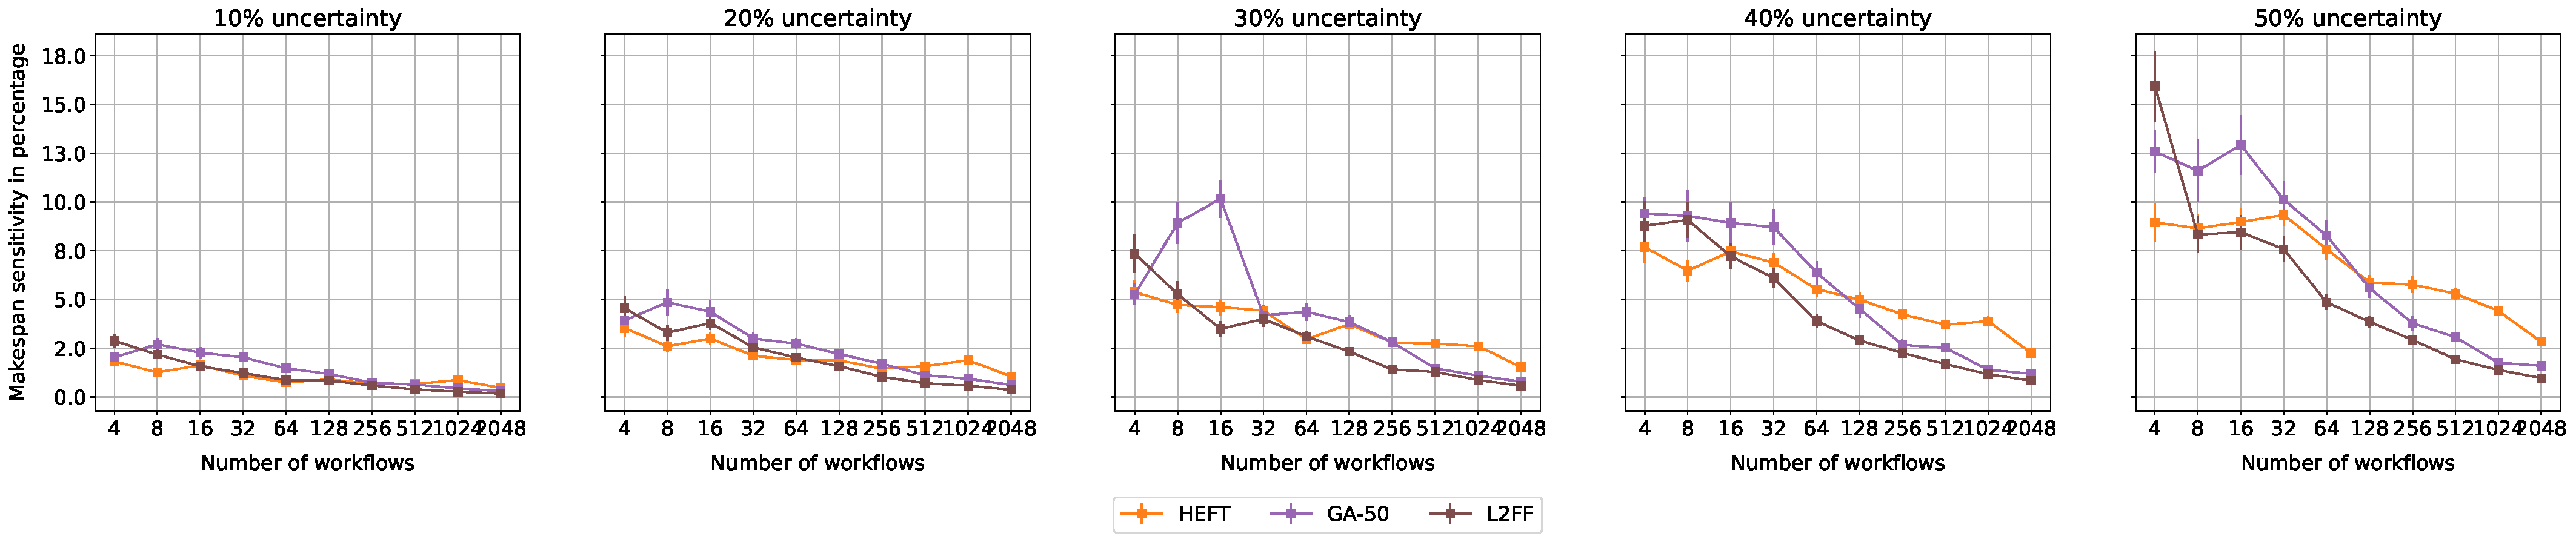
\includegraphics[width=.95\textwidth]{figures/campaign/InaccurStHeteroCampaigns_4StHeteroResourcesSens.pdf}
        \caption{}
        \label{fig:InaccurStHeteroCampaigns_4StHeteroResourcesSens}
    \end{subfigure}\\
    ~
    \begin{subfigure}[b]{0.95\textwidth}
        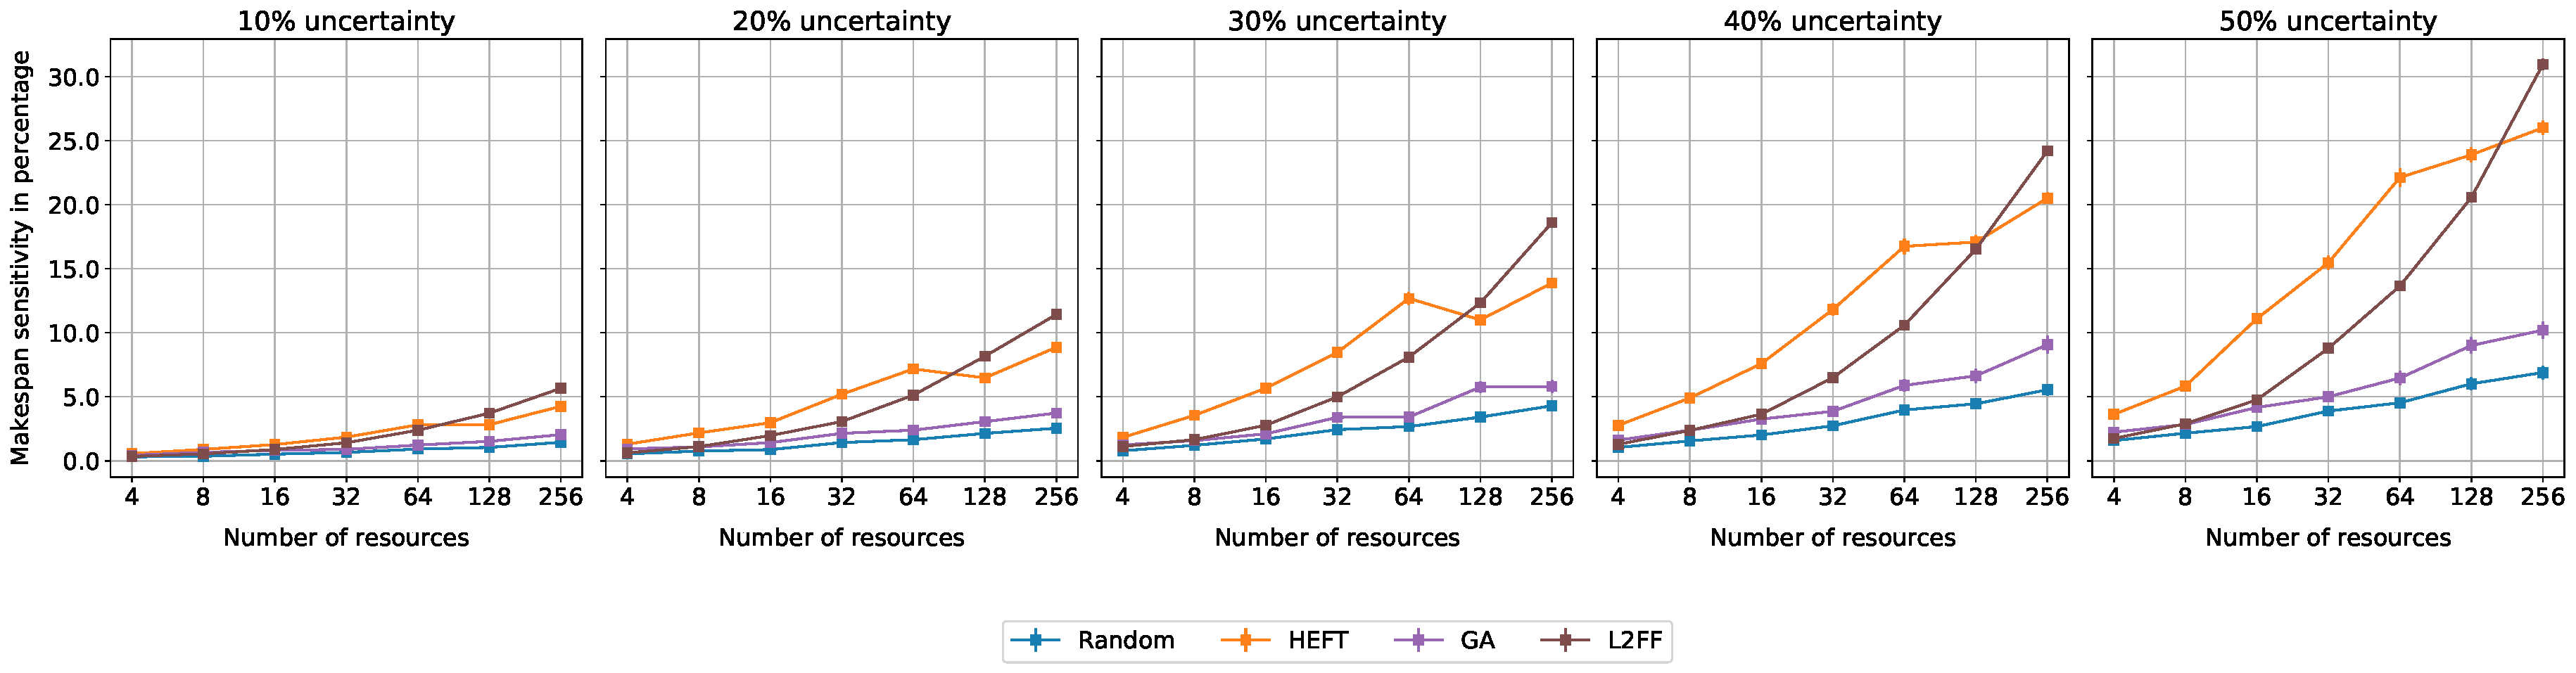
\includegraphics[width=0.95\textwidth]{figures/campaign/InaccurStHeteroResources_StHeteroCampaignsSens.pdf}
        \caption{}
        \label{fig:InaccurStHeteroResources_StHeteroCampaignsSens}
    \end{subfigure}
    \caption{~\ref{fig:InaccurStHeteroCampaigns_4StHeteroResourcesSens} Makespan
    sensitivity for different levels of uncertainty and different number of
    workflows on 4 heterogeneous resources;
    \ref{fig:InaccurStHeteroResources_StHeteroCampaignsSens} Makespan
    sensitivity for different levels of uncertainty and different number of
    resources for 1024 workflows static resources.}
    \label{fig:inaccur_st}
\end{figure}

As per our expectation, sensitivity to workflow uncertainty decreases when the
number of workflows increase
(Fig.~\ref{fig:InaccurStHeteroCampaigns_4StHeteroResourcesSens}) and increases
as the number of resources increase
(Fig.~\ref{fig:InaccurStHeteroResources_StHeteroCampaignsSens}). This result,
along with experiment 2, let us to conclude that as the average number of
workflows per resource increases, the sensitivity value will decrease.

Sensitivity to makespan runtime uncertainty shows a wide range of values for
HEFT and L2FF, but a significantly smaller range for GA and Random.
Specifically, the sensitivity of plans using HEFT is between almost 0~\% for
2048 workflows on 4 resource and 25~\% for 1024 workflows on 256 resources. The
sensitivity of plans using L2FF show a similar range to the one seen when using
HEFT, with L2FF reaching 35~\% for 1024 workflows on 256 resources. GA plans
show increased sensitivity for a small number of workflows when the number of
resources is constant ($\approx$13~\%), and quickly drop close to 0~\%.

HEFT ranks and L2FF sorts all the workflows based on runtime information, while
GA uses that information only to map 50\% of the workflows of each plan to
resources, for each generation. When the runtime information is uncertain, any
type of ordering will not necessarily be correct as the runtime estimation is
not the same as the actual runtime. Since GA utilizes such information for half
of the workflows at every generation, while the other half is placed on
resources randomly, GA is less sensitive to workflow runtime uncertainty than
HEFT and L2FF.

HEFT shows higher sensitivity than GA and L2FF above 128 workflows and 4
resources, and when the number of resources changes with 1024 workflows. In
addition, we see higher sensitivity for plans that use HEFT and L2FF than plans
that use GA when the number of resources increases. Both HEFT and L2FF create
priority lists for the workflows and GA does not. As a result, HEFT and L2FF
place large workflows on less performant resources. GA does not prioritize
workflows and places a subset of workflows to resources randomly. As a
consequence, the random order of the workflows with the random placement reduces
the effect of the workflow runtime uncertainty.

We conclude that algorithms like HEFT and L2FF that prioritize workflows tend to
be more sensitive to workflow runtime estimation uncertainty than algorithms
that do not create a priority list, such as GA and Random. Workflow runtime
uncertainty can make the order decided by HEFT and L2FF invalid and, as a
result, long workflow may be placed on less performant resource, increasing
makespan. HEFT and L2FF are more sensitive than GA and random when the number of
resources increases: 25~\% and 35~\% compared to less than 10~\% for 1024
workflows and 256 resources. Further, all algorithms show similar sensitivity
when the number of workflows increases. Sensitivity remains proportional to the
number of resources and inverse proportional to the number of workflows. This,
in conjunction to the results of experiment 2, allows us to conclude that the
sensitivity slope is independent of the type of uncertainty.

\section{Conclusions}
\label{sec:cf_algo_sel}

In this chapter, we discuss and compare algorithms to plan the execution of a
computational campaign on HPC resources. Specifically, we discuss the
characteristics of three planning algorithms: HEFT, GA and L2FF. Our
experimental methodology allows us to compare plans in terms of makespan
performance, and their sensitivity to resource dynamism and workflow runtime
uncertainty.

Our analysis shows that there are three algorithmic properties which affect the
performance and sensitivity of planning algorithms. The first property is
whether the algorithm estimates resource availability. HEFT and GA estimate when
resources are available and show better makespan performance on homogeneous and
heterogeneous resources than L2FF and random. The second property is whether the
algorithm uses a deterministic or randomized heuristic to place workflows on
resources. GA shows performance similar to random plans when all workflows were
initially placed randomly to resources. In addition, when using more than 128
resources, GA-50 shows worse performance than L2Ff as it underutilized some of
the resources. The third property is whether the algorithm creates a workflow
priority list based on workflow runtime. HEFT and L2FF sort workflows based on
their runtime, placing first the longer workflows on their lists. This priority
list allows L2FF to place longer workflows to more performant resources and, as
a result, L2Ff outperforms GA with more than \mtnote{add number of resources
here} resources.

Our analysis of the makespan sensitivity shows that deterministic algorithms are
more sensitive to resource dynamism or workflow runtime uncertainty than
non-deterministic algorithms. HEFT and L2FF provide more sensitive plans than GA
and Random. Further, sensitivity is proportional to the number of resources and
inverse proportional to the number of workflows. Sensitivity to resource
dynamism or workflow runtime uncertainty: (1) decreases as the number of
workflows increases and the number of resources is constant ; and (2) increases
when number of resources increases and the number of workflows is constant. Both
HEFT and L2FF are more sensitive to workflow runtime uncertainty than GA since
they prioritize workflows based on their runtime estimation.

We conclude that users should select different planning algorithms to derive an
execution plan, depending on the properties of the campaign and resources. When
resources are homogeneous, a planner like L2FF provides a plan with good
makespan, is very simple to engineer and is not significantly more sensitive
than algorithms like HEFT or GA. When resources are heterogeneous and the
computational objective is to produce the best possible makespan, an
deterministic algorithm like HEFT that derive information about resource
availability and creates a priority list is a better candidate. If the objective
of a campaign is to use a plan that is not very sensitive to resource dynamism
or workflow runtime uncertainty, a non-deterministic algorithm like GA is a
better candidate than the other two types of algorithms. Although GA may provide
plans with worse makespan than an algorithm like HEFT, its plans are less
sensitive to workflow runtime uncertainty.


%% --------------------------------- OLD TEXT ----------------------------------

%% ---------------------------- HEFT EXTENSION ---------------------------------
%HPC resources may become unavailable for multiple reasons, including but not limited to maintenance, a random failure, executing a workflows over the expected time., etc.
%In order to be able to utilize HEFT for dynamic resources, we had to extend Algorithm~\ref{alg:heft} to take as input the time that a resource is initially available.
%This input can be represented as a dictionary where the keys are the available resources and the values are the time a resource becomes available.
%The extended algorithm is shown in Algorithm~\ref{alg:ext_heft}.
%Although the extension may be small, it is crucial to allow to reuse HEFT based on the state of the execution at a given point in time.
%
%\begin{algorithm}[ht]
%    \caption{Extended Heterogeneous Earliest Finish Time (EHEFT) algorithm}
%    \label{alg:ext_heft}
%    \begin{algorithmic}[1]
%        \Procedure{EHEFT}{$W$, $R$, $T$}\Comment{$W$ and $R$ are a set of workflow and resources respectively. $T$ is a dictionary of when a resource becomes available.}
%        \State \texttt{Calculate the computation cost $w_{tx}^{ij}$ of each workflow for all resources}
%        \State \texttt{Assign $rank_i = \overline{w_{i}} = \nicefrac{\sum_{j=1}^{|R|}w_{tx}^{ij}}{|R|}$}
%        \State \texttt{Sort workflows by non-increasing order of $rank_i$}
%        \While{unscheduled workflows}
%        \State \texttt{Select the first workflow $\tilde{w}$ from the sorted list}
%        \For{$\forall r_{j}$ in $R$}
%        \State\texttt{Compute earliest finish time for $\tilde{w}$ on $r_{j}$ based on $T(r_j)$, $eft_{\tilde{w},r_j}$ }
%        \EndFor
%        \State \texttt{Assign  $\tilde{w}$ on $r_k$ with $\min{(eft_{\tilde{w},r_j})}$}
%        \EndWhile
%        \EndProcedure
%    \end{algorithmic}
%\end{algorithm}
%

%% -------------------- GA EXTENSION -------------------------------------------
%We extend this algorithm in the population initialization to support replanning..
%The initialization method takes into account the times resources will be available during for the EFT heuristic.
%Another point of extension would be the fitness function.
%However, the fitness function of the selected algorithm~\cite{page2005algorithm} already takes into account the previous load of a resource, which is the time a resource is available.

%% -----------------------------------------------------------------------------
%In figure~\ref{fig:dyn_hetero_homog_sens_analysis} we introduce workflow heterogeneity.
%The algorithms makespan performance behavior is similar to the one shown in Fig.~\ref{fig:het_het_analysis}.
%Despite the fact, HEFT show the largest sensitivity when varying the number of workflows and when varying the number of resources.
%The genetic algorithm shows similar sensitivity with HEFT when the number of workflows but tends to be less sensitive when the number of resources increase.
%The genetic algorithm assigns a percentage of workflows to resources randomly which in turn makes it less sensitive to resource dynamicity, especially when the number of resources is large.

%L2FF shows a similar behavior with HEFT, especially when the number of resources changes, despite being less sensitive.
%In addition, the genetic algorithm sensitivity gets closer to that of random when the number of resources increases.
%Both L2FF and HEFT are deterministic and they produce always the same plan for a given campaign and set of resources.
%This in turn results to an increasing sensitivity as the ratio of number of campaign size to number of resources is small.
%In contrast, the random initial placement of GA allows it to create a plan that is less sensitive to dynamicity with the cost of slightly makespan, 725K seconds versus 643K and 649K seconds from HEFT and L2FF respectively.

%% -----------------------------------------------------------------------------
% Experiment 3 dynamic resources
%
%The ratio of number of workflows over the number of resources remains inverse proportional to the sensitivity.
%In addition, specifically for HEFT the impact of uncertainty increases significantly as the number of resources increase, reaching 55~\%.
%Since HEFT places one or two workflows on these resources, any change affects significantly its expected makespan.
%This verifies our conclusion from experiment 2, that algorithms with strong assumptions about workflow runtime and resource availability are very sensitive to changes.
%
%Introducing resource dynamism increased further the sensitivity of the algorithms, as seen in figure~\ref{fig:inaccur_dyn}.
%The observed increase was no more than the level shown in experiment 2.
%This shows us that the overall sensitivity is the summation of independently measured sensitivity from different sources.
%
%The results of our experiments show that algorithms which make significant assumptions about the workflow length and resource performance produce better makespan.
%That is apparent from the fact that HEFT consistently produces the smaller makespan.
%This is true also when resources are dynamic and the workflows runtime is uncertain even at 90~\%.
%HEFT had a sensitivity of around 60~\% maximum which is not enough to affect the plan in such a way that another algorithm would be preferable.
%Furthermore, knowledge of resource heterogeneity and availability is an important factor in differentiating the performance of the algorithms, as seen by the performance difference of L2FF compared to HEFT and GA.
%Lastly, the ratio of the number of workflows over the number of resources affects the level of sensitivity of the algorithms.
%The less number of workflows placed on resources higher the significance of a change either in the performance of the resources or the workflow runtime.
%

%% -----------------------------------------------------------------------------
%
%\subsection{Experiment 4: Performance Gain using Plan Adaptation}
%
%An adaptive plan is a new plan derived from the previous one on the base of information acquired at runtime.
%Plan adaptation can happen either via running the planning algorithm again with the new information or via submitting a workflow to the selected resource when it becomes available.
%In this experiment, we focus on the second type of adaptation since L2FF does not know when exactly a resource becomes available.
%Specifically, when a resource becomes available earlier than expected, the bookkeeping component pushes the next workflow to the selected resource, otherwise the workflow is queued and executes as soon the resource becomes available.
%
%We measure the performance gain of adaptive plans for executing a campaign with heterogeneous workflows and different level of uncertainty on heterogeneous dynamic resources.
%Figure~\ref{fig:gain_dyn} shows the normalized performance gain as a function of the workflow runtime uncertainty and either the number of workflows, fig.~\ref{fig:InaccurStHeteroCampaigns_4DynHeteroResourcesGain}, or the number of resources, fig.~\ref{fig:InaccurDynHeteroResources_StHeteroCampaignsGain}.
%As we can see the performance gain is not significant.
%L2FF adaptive plan shows a maximum of 16~\% for 4 workflows and 4 resources, GA and HEFT around 12~\%, while when the number of resources vary none of the plans exceeds 6~\%.
%
%
%\begin{figure}[ht!]
%    \centering
%    \begin{subfigure}[b]{0.95\textwidth}
%        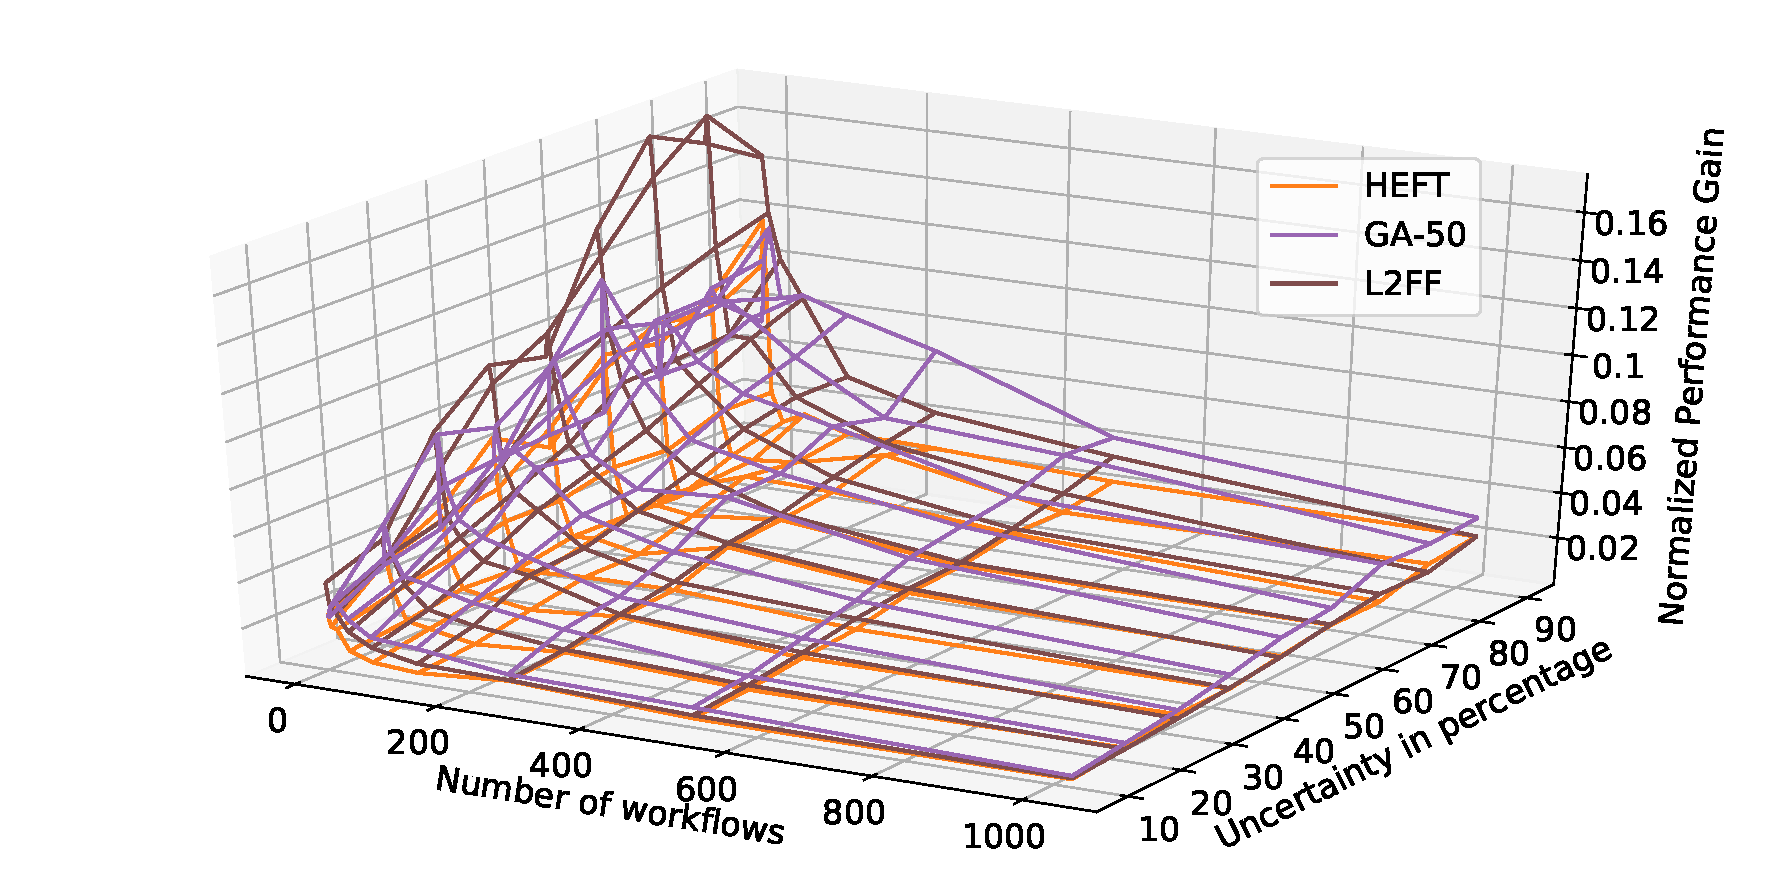
\includegraphics[width=.95\textwidth]{figures/campaign/InaccurStHeteroCampaigns_4DynHeteroResourcesGain.pdf}
%        \caption{}
%        \label{fig:InaccurStHeteroCampaigns_4DynHeteroResourcesGain}
%    \end{subfigure}\\
%    ~
%    \begin{subfigure}[b]{0.95\textwidth}
%        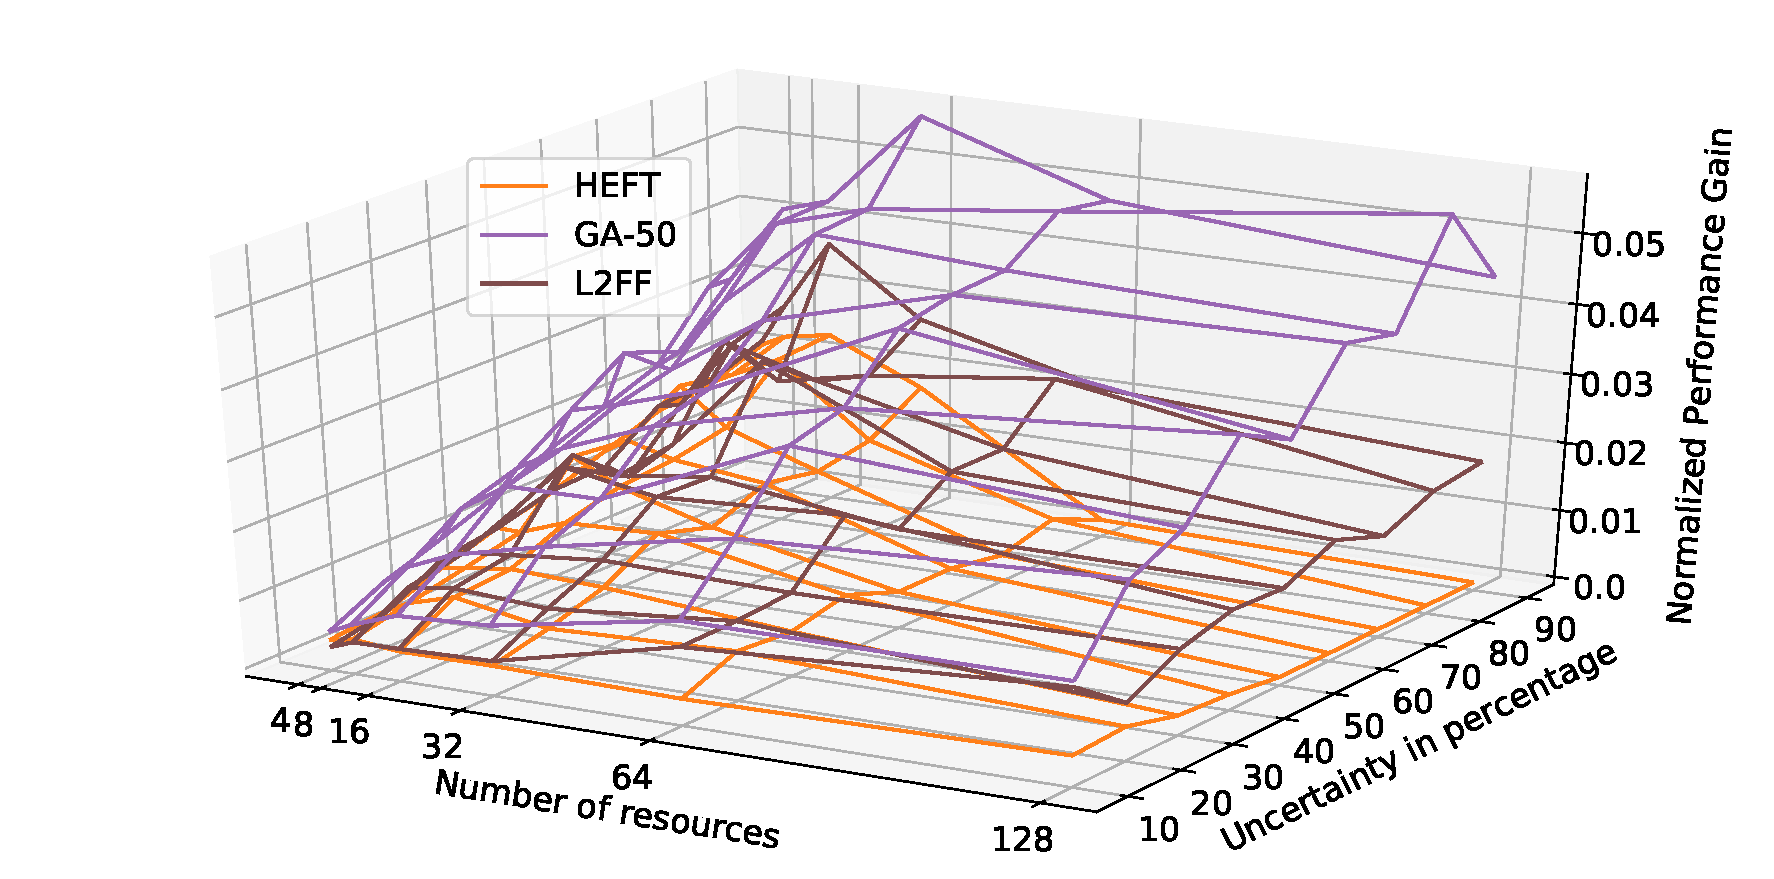
\includegraphics[width=0.95\textwidth]{figures/campaign/InaccurDynHeteroResources_StHeteroCampaignsGain.pdf}
%        \caption{}
%        \label{fig:InaccurDynHeteroResources_StHeteroCampaignsGain}
%    \end{subfigure}
%    \caption{~\ref{fig:InaccurStHeteroCampaigns_4DynHeteroResourcesGain} Normalized performance gain for different levels of uncertainty and different number of workflows on static resources;
%        ~\ref{fig:InaccurDynHeteroResources_StHeteroCampaignsGain} Normalized performance gain for different levels of uncertainty and different number of resources on static resources.}
%    \label{fig:gain_dyn}
%\end{figure}
%
%Since adaptive plans try to mitigate the effects of resource dynamism and workflow runtime uncertainty, we expect that the performance gain would be proportional to the ratio of number of workflows over the number of resources.
%Although this is generally true for L2FF and GA, it is not for HEFT.
%This is due to the fact that HEFT is placing a small number, 1 or 2, of workflows on slow resources.
%As a result, adaptive plans have no or very little effect.
%Contrary, L2FF and GA place more workflows on the slow resources allowing the adaptation to provide some gains.


%% --------------------------- Last Experiment ---------------------------------

%\begin{figure}[ht!]
%    \centering
%    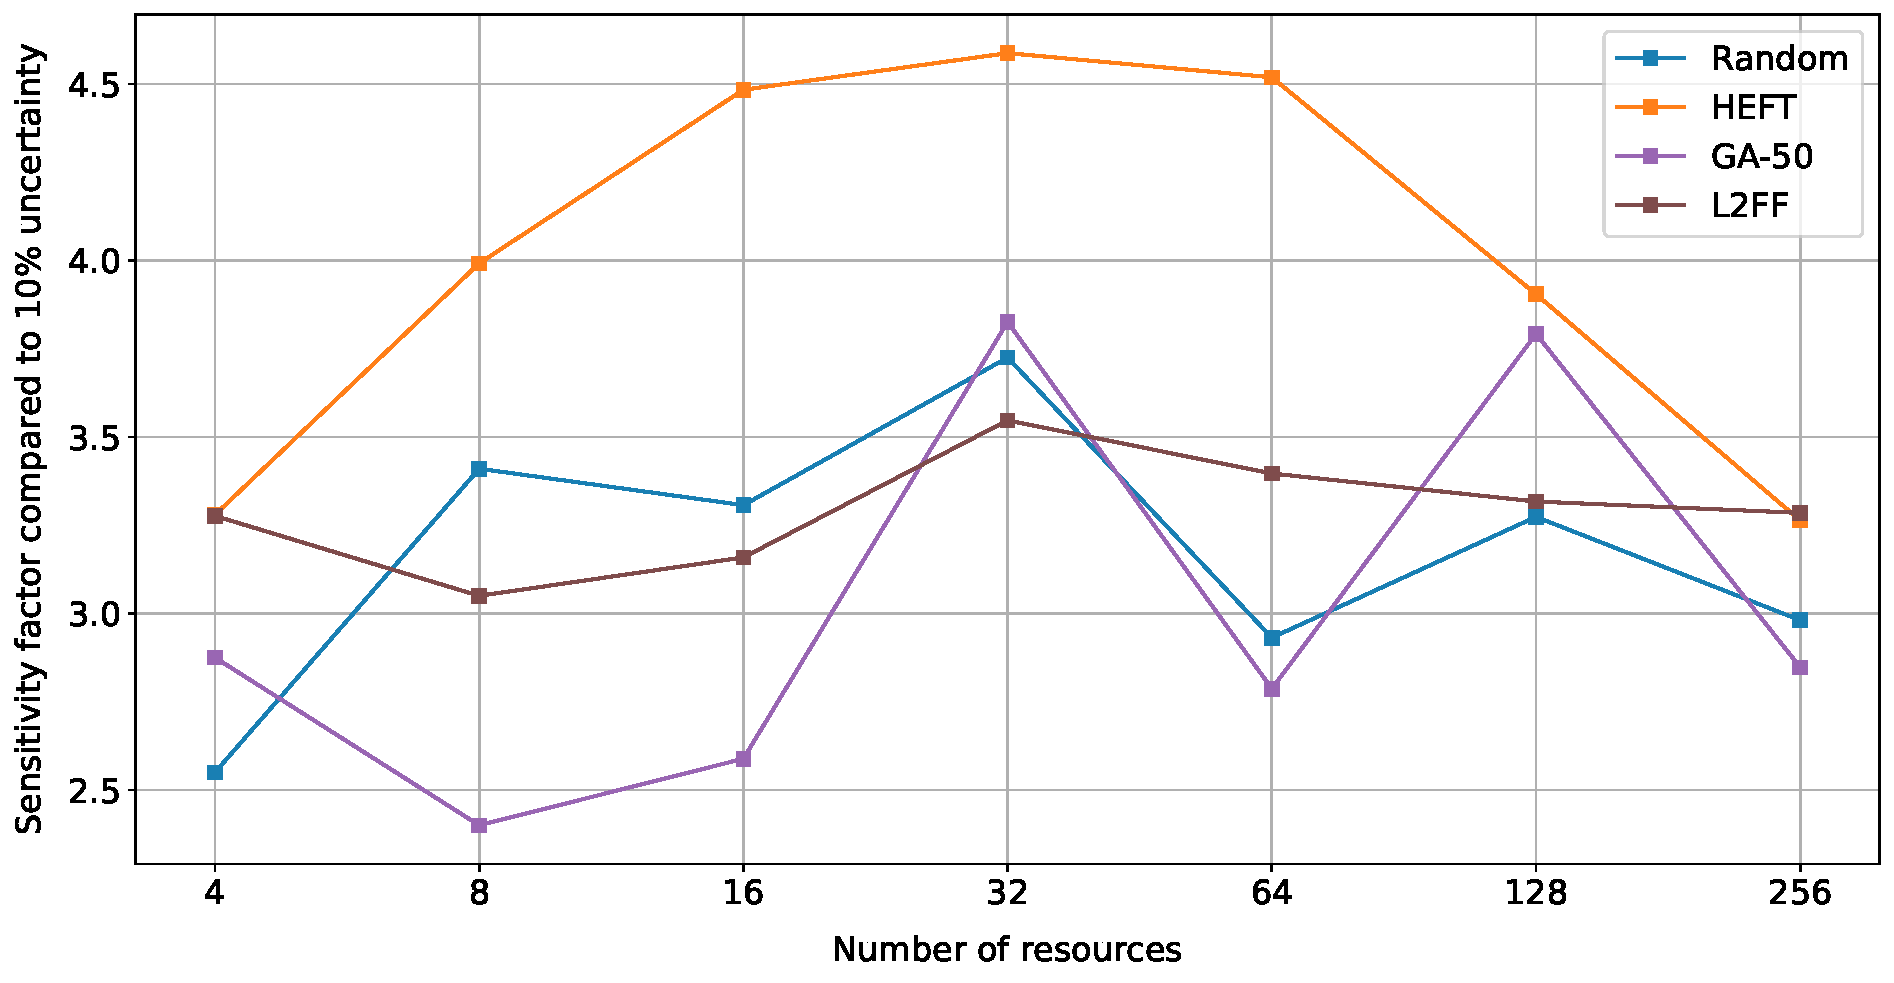
\includegraphics[width=.95\textwidth]{figures/campaign/InaccurStHeteroResources_StHeteroCampaignsSensFactor.pdf}
%    \caption{Sensitivity factor for 30~\% uncertainty compared to 10~\% uncertainty for different number of resources and 1024 workflows.}
%    \label{fig:InaccurStHeteroResources_StHeteroCampaignsSensFactor}
%\end{figure}

%As the level of uncertainty increases the sensitivity increases proportionally for L2FF and GA and not for HEFT regardless of whether the number of workflows or the number of resources changes.
%HEFT shows an increase larger than the expected multiplicative factor when the number of workflows over the number of resources is between 8 and 128.
%As an example, figure~\ref{fig:InaccurStHeteroResources_StHeteroCampaignsSensFactor} shows the increase factor of 30~\% uncertainty compared to 10~\% for different number of resources and 1024 workflows.
%L2FF, GA and random increase is relatively close to 3 compared to the increase observed for HEFT which reaches more than 4 times.
%We believe that this unexpected behavior from HEFT is a consequence of prioritizing workflows and placing a workflow on the resource that will finish it earlier.